\documentclass[1p]{elsarticle_modified}
%\bibliographystyle{elsarticle-num}

%\usepackage[colorlinks]{hyperref}
%\usepackage{abbrmath_seonhwa} %\Abb, \Ascr, \Acal ,\Abf, \Afrak
\usepackage{amsfonts}
\usepackage{amssymb}
\usepackage{amsmath}
\usepackage{amsthm}
\usepackage{scalefnt}
\usepackage{amsbsy}
\usepackage{kotex}
\usepackage{caption}
\usepackage{subfig}
\usepackage{color}
\usepackage{graphicx}
\usepackage{xcolor} %% white, black, red, green, blue, cyan, magenta, yellow
\usepackage{float}
\usepackage{setspace}
\usepackage{hyperref}

\usepackage{tikz}
\usetikzlibrary{arrows}

\usepackage{multirow}
\usepackage{array} % fixed length table
\usepackage{hhline}

%%%%%%%%%%%%%%%%%%%%%
\makeatletter
\renewcommand*\env@matrix[1][\arraystretch]{%
	\edef\arraystretch{#1}%
	\hskip -\arraycolsep
	\let\@ifnextchar\new@ifnextchar
	\array{*\c@MaxMatrixCols c}}
\makeatother %https://tex.stackexchange.com/questions/14071/how-can-i-increase-the-line-spacing-in-a-matrix
%%%%%%%%%%%%%%%

\usepackage[normalem]{ulem}

\newcommand{\msout}[1]{\ifmmode\text{\sout{\ensuremath{#1}}}\else\sout{#1}\fi}
%SOURCE: \msout is \stkout macro in https://tex.stackexchange.com/questions/20609/strikeout-in-math-mode

\newcommand{\cancel}[1]{
	\ifmmode
	{\color{red}\msout{#1}}
	\else
	{\color{red}\sout{#1}}
	\fi
}

\newcommand{\add}[1]{
	{\color{blue}\uwave{#1}}
}

\newcommand{\replace}[2]{
	\ifmmode
	{\color{red}\msout{#1}}{\color{blue}\uwave{#2}}
	\else
	{\color{red}\sout{#1}}{\color{blue}\uwave{#2}}
	\fi
}

\newcommand{\Sol}{\mathcal{S}} %segment
\newcommand{\D}{D} %diagram
\newcommand{\A}{\mathcal{A}} %arc


%%%%%%%%%%%%%%%%%%%%%%%%%%%%%5 test

\def\sl{\operatorname{\textup{SL}}(2,\Cbb)}
\def\psl{\operatorname{\textup{PSL}}(2,\Cbb)}
\def\quan{\mkern 1mu \triangleright \mkern 1mu}

\theoremstyle{definition}
\newtheorem{thm}{Theorem}[section]
\newtheorem{prop}[thm]{Proposition}
\newtheorem{lem}[thm]{Lemma}
\newtheorem{ques}[thm]{Question}
\newtheorem{cor}[thm]{Corollary}
\newtheorem{defn}[thm]{Definition}
\newtheorem{exam}[thm]{Example}
\newtheorem{rmk}[thm]{Remark}
\newtheorem{alg}[thm]{Algorithm}

\newcommand{\I}{\sqrt{-1}}
\begin{document}

%\begin{frontmatter}
%
%\title{Boundary parabolic representations of knots up to 8 crossings}
%
%%% Group authors per affiliation:
%\author{Yunhi Cho} 
%\address{Department of Mathematics, University of Seoul, Seoul, Korea}
%\ead{yhcho@uos.ac.kr}
%
%
%\author{Seonhwa Kim} %\fnref{s_kim}}
%\address{Center for Geometry and Physics, Institute for Basic Science, Pohang, 37673, Korea}
%\ead{ryeona17@ibs.re.kr}
%
%\author{Hyuk Kim}
%\address{Department of Mathematical Sciences, Seoul National University, Seoul 08826, Korea}
%\ead{hyukkim@snu.ac.kr}
%
%\author{Seokbeom Yoon}
%\address{Department of Mathematical Sciences, Seoul National University, Seoul, 08826,  Korea}
%\ead{sbyoon15@snu.ac.kr}
%
%\begin{abstract}
%We find all boundary parabolic representation of knots up to 8 crossings.
%
%\end{abstract}
%\begin{keyword}
%    \MSC[2010] 57M25 
%\end{keyword}
%
%\end{frontmatter}

%\linenumbers
%\tableofcontents
%
\newcommand\colored[1]{\textcolor{white}{\rule[-0.35ex]{0.8em}{1.4ex}}\kern-0.8em\color{red} #1}%
%\newcommand\colored[1]{\textcolor{white}{ #1}\kern-2.17ex	\textcolor{white}{ #1}\kern-1.81ex	\textcolor{white}{ #1}\kern-2.15ex\color{red}#1	}

{\Large $\underline{12a_{0847}~(K12a_{0847})}$}

\setlength{\tabcolsep}{10pt}
\renewcommand{\arraystretch}{1.6}
\vspace{1cm}\begin{tabular}{m{100pt}>{\centering\arraybackslash}m{274pt}}
\multirow{5}{120pt}{
	\centering
	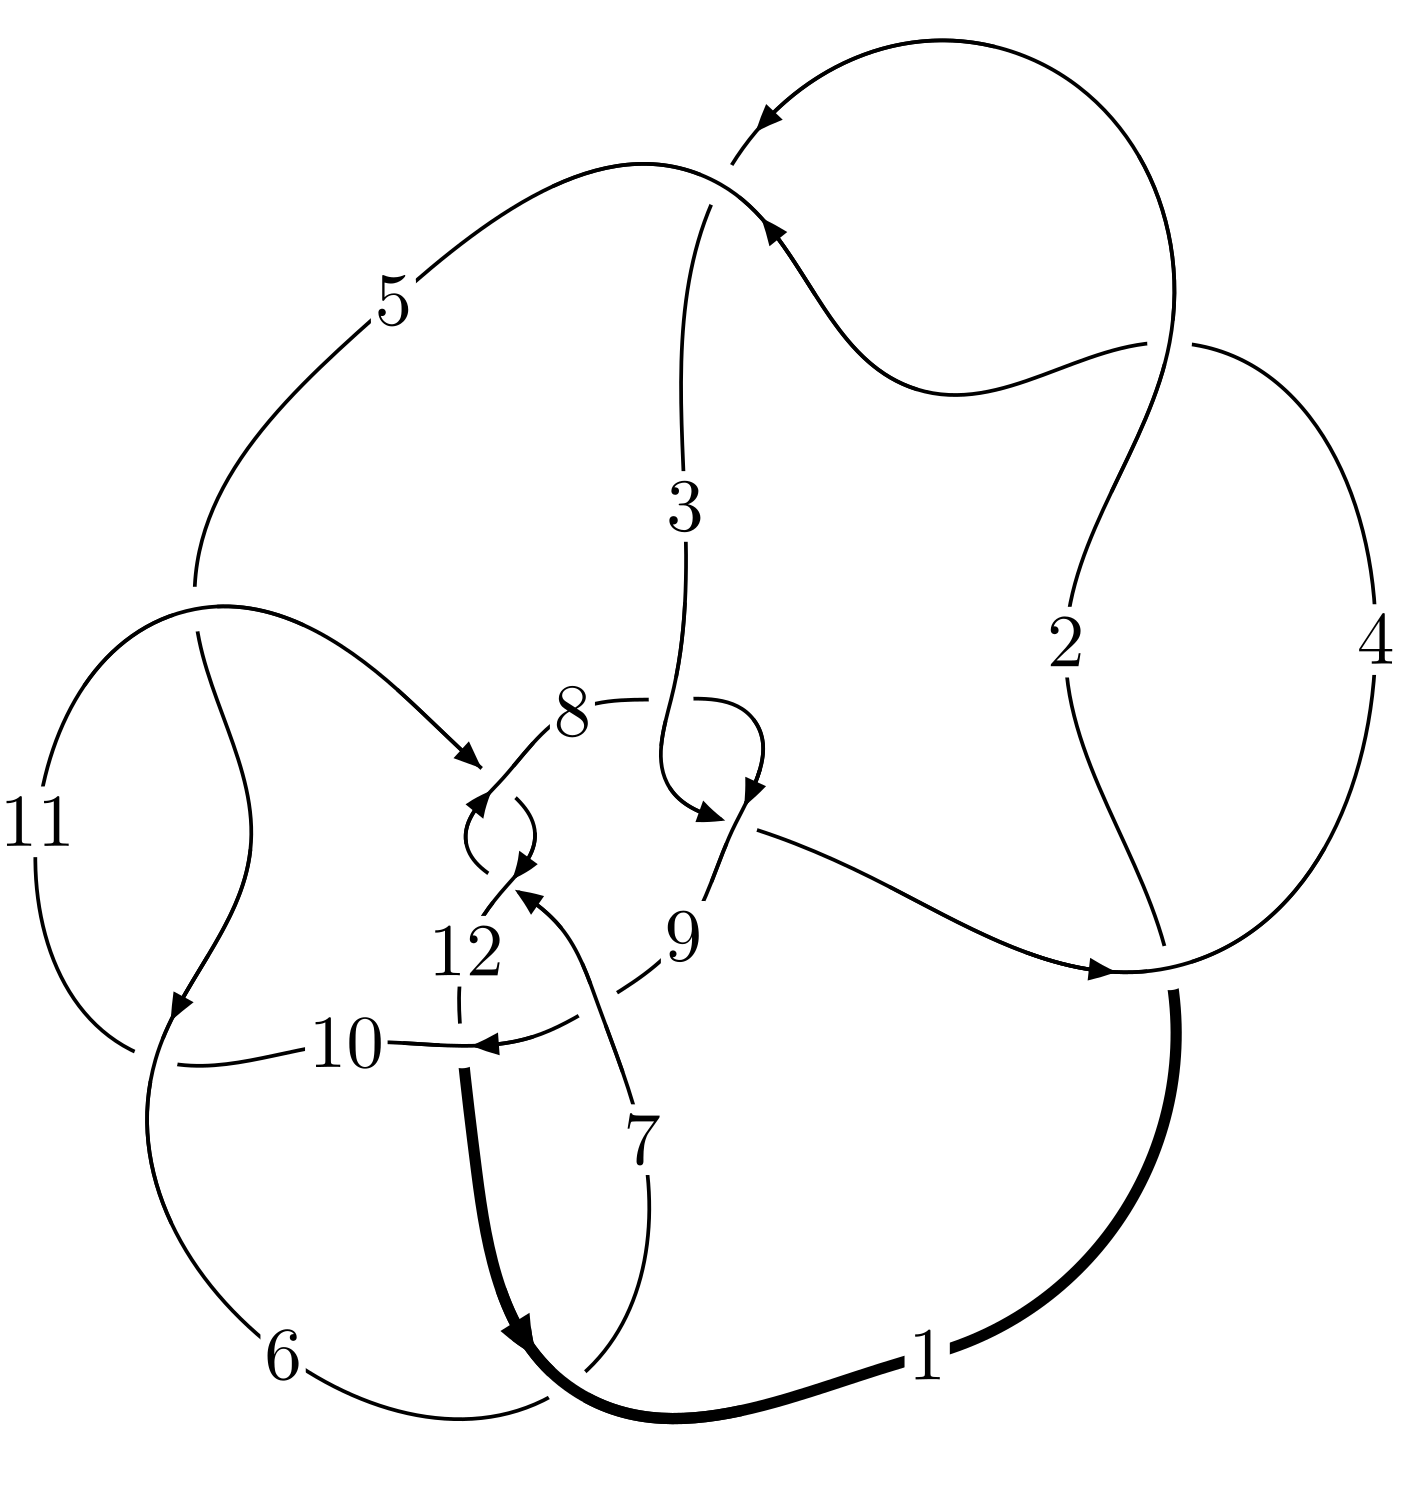
\includegraphics[width=112pt]{../../../GIT/diagram.site/Diagrams/png/1648_12a_0847.png}\\
\ \ \ A knot diagram\footnotemark}&
\allowdisplaybreaks
\textbf{Linearized knot diagam} \\
\cline{2-2}
 &
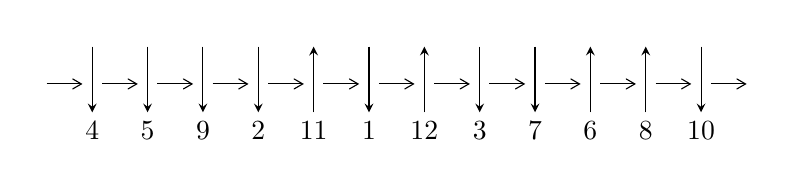
\begin{tikzpicture}[x=20pt, y=17pt]
	% nodes
	\node (C0) at (0, 0) {};
	\node (C1) at (1, 0) {};
	\node (C1U) at (1, +1) {};
	\node (C1D) at (1, -1) {4};

	\node (C2) at (2, 0) {};
	\node (C2U) at (2, +1) {};
	\node (C2D) at (2, -1) {5};

	\node (C3) at (3, 0) {};
	\node (C3U) at (3, +1) {};
	\node (C3D) at (3, -1) {9};

	\node (C4) at (4, 0) {};
	\node (C4U) at (4, +1) {};
	\node (C4D) at (4, -1) {2};

	\node (C5) at (5, 0) {};
	\node (C5U) at (5, +1) {};
	\node (C5D) at (5, -1) {11};

	\node (C6) at (6, 0) {};
	\node (C6U) at (6, +1) {};
	\node (C6D) at (6, -1) {1};

	\node (C7) at (7, 0) {};
	\node (C7U) at (7, +1) {};
	\node (C7D) at (7, -1) {12};

	\node (C8) at (8, 0) {};
	\node (C8U) at (8, +1) {};
	\node (C8D) at (8, -1) {3};

	\node (C9) at (9, 0) {};
	\node (C9U) at (9, +1) {};
	\node (C9D) at (9, -1) {7};

	\node (C10) at (10, 0) {};
	\node (C10U) at (10, +1) {};
	\node (C10D) at (10, -1) {6};

	\node (C11) at (11, 0) {};
	\node (C11U) at (11, +1) {};
	\node (C11D) at (11, -1) {8};

	\node (C12) at (12, 0) {};
	\node (C12U) at (12, +1) {};
	\node (C12D) at (12, -1) {10};
	\node (C13) at (13, 0) {};

	% arrows
	\draw[->,>={angle 60}]
	(C0) edge (C1) (C1) edge (C2) (C2) edge (C3) (C3) edge (C4) (C4) edge (C5) (C5) edge (C6) (C6) edge (C7) (C7) edge (C8) (C8) edge (C9) (C9) edge (C10) (C10) edge (C11) (C11) edge (C12) (C12) edge (C13) ;	\draw[->,>=stealth]
	(C1U) edge (C1D) (C2U) edge (C2D) (C3U) edge (C3D) (C4U) edge (C4D) (C5D) edge (C5U) (C6U) edge (C6D) (C7D) edge (C7U) (C8U) edge (C8D) (C9U) edge (C9D) (C10D) edge (C10U) (C11D) edge (C11U) (C12U) edge (C12D) ;
	\end{tikzpicture} \\
\hhline{~~} \\& 
\textbf{Solving Sequence} \\ \cline{2-2} 
 &
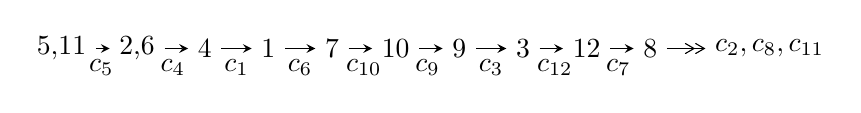
\begin{tikzpicture}[x=23pt, y=7pt]
	% node
	\node (A0) at (-1/8, 0) {5,11};
	\node (A1) at (17/16, 0) {2,6};
	\node (A2) at (17/8, 0) {4};
	\node (A3) at (25/8, 0) {1};
	\node (A4) at (33/8, 0) {7};
	\node (A5) at (41/8, 0) {10};
	\node (A6) at (49/8, 0) {9};
	\node (A7) at (57/8, 0) {3};
	\node (A8) at (65/8, 0) {12};
	\node (A9) at (73/8, 0) {8};
	\node (C1) at (1/2, -1) {$c_{5}$};
	\node (C2) at (13/8, -1) {$c_{4}$};
	\node (C3) at (21/8, -1) {$c_{1}$};
	\node (C4) at (29/8, -1) {$c_{6}$};
	\node (C5) at (37/8, -1) {$c_{10}$};
	\node (C6) at (45/8, -1) {$c_{9}$};
	\node (C7) at (53/8, -1) {$c_{3}$};
	\node (C8) at (61/8, -1) {$c_{12}$};
	\node (C9) at (69/8, -1) {$c_{7}$};
	\node (A10) at (11, 0) {$c_{2},c_{8},c_{11}$};

	% edge
	\draw[->,>=stealth]	
	(A0) edge (A1) (A1) edge (A2) (A2) edge (A3) (A3) edge (A4) (A4) edge (A5) (A5) edge (A6) (A6) edge (A7) (A7) edge (A8) (A8) edge (A9) ;
	\draw[->>,>={angle 60}]	
	(A9) edge (A10);
\end{tikzpicture} \\ 

\end{tabular} \\

\footnotetext{
The image of knot diagram is generated by the software ``\textbf{Draw programme}" developed by Andrew Bartholomew(\url{http://www.layer8.co.uk/maths/draw/index.htm\#Running-draw}), where we modified some parts for our purpose(\url{https://github.com/CATsTAILs/LinksPainter}).
}\phantom \\ \newline 
\centering \textbf{Ideals for irreducible components\footnotemark of $X_{\text{par}}$} 
 
\begin{align*}
I^u_{1}&=\langle 
3.31232\times10^{25} u^{39}-1.32076\times10^{25} u^{38}+\cdots+2.23057\times10^{24} b+8.08236\times10^{25},\\
\phantom{I^u_{1}}&\phantom{= \langle  }6.20649\times10^{25} u^{39}-3.16207\times10^{25} u^{38}+\cdots+4.46114\times10^{24} a+1.24112\times10^{26},\;u^{40}+16 u^{38}+\cdots+7 u+1\rangle \\
I^u_{2}&=\langle 
1.14706\times10^{193} u^{65}+1.22942\times10^{193} u^{64}+\cdots+3.43598\times10^{195} b+3.53438\times10^{197},\\
\phantom{I^u_{2}}&\phantom{= \langle  }2.71067\times10^{205} u^{65}-5.82931\times10^{205} u^{64}+\cdots+1.90669\times10^{207} a-8.28943\times10^{207},\\
\phantom{I^u_{2}}&\phantom{= \langle  }u^{66}-2 u^{65}+\cdots+34394 u+12919\rangle \\
I^u_{3}&=\langle 
4 u^{19}-2 u^{18}+\cdots+b-11,\;3 u^{19}+u^{18}+\cdots+a-7,\;u^{20}+10 u^{18}+\cdots-3 u+1\rangle \\
I^u_{4}&=\langle 
b+1,\;- u^3+u^2+2 a- u+1,\;u^4+u^2+u+1\rangle \\
I^u_{5}&=\langle 
-1211 u^{11}-823 u^{10}+\cdots+3595 b-1417,\;41974 u^{11}+28420 u^{10}+\cdots+17975 a+80569,\\
\phantom{I^u_{5}}&\phantom{= \langle  }u^{12}+u^{11}+6 u^{10}+8 u^9+18 u^8+22 u^7+33 u^6+32 u^5+40 u^4+28 u^3+25 u^2+8 u+1\rangle \\
I^u_{6}&=\langle 
- u^5+u^4+u^2+b-1,\;- u^5+u^4- u^3+u^2+a- u,\;u^6- u^5+u^4-2 u^3+u^2+1\rangle \\
I^u_{7}&=\langle 
b+1,\;u^5+2 u^3+a+u,\;u^6- u^5+2 u^4-2 u^3+2 u^2-2 u+1\rangle \\
\\
\end{align*}
\raggedright * 7 irreducible components of $\dim_{\mathbb{C}}=0$, with total 154 representations.\\
\footnotetext{All coefficients of polynomials are rational numbers. But the coefficients are sometimes approximated in decimal forms when there is not enough margin.}
\newpage
\renewcommand{\arraystretch}{1}
\centering \section*{I. $I^u_{1}= \langle 3.31\times10^{25} u^{39}-1.32\times10^{25} u^{38}+\cdots+2.23\times10^{24} b+8.08\times10^{25},\;6.21\times10^{25} u^{39}-3.16\times10^{25} u^{38}+\cdots+4.46\times10^{24} a+1.24\times10^{26},\;u^{40}+16 u^{38}+\cdots+7 u+1 \rangle$}
\flushleft \textbf{(i) Arc colorings}\\
\begin{tabular}{m{7pt} m{180pt} m{7pt} m{180pt} }
\flushright $a_{5}=$&$\begin{pmatrix}1\\0\end{pmatrix}$ \\
\flushright $a_{11}=$&$\begin{pmatrix}0\\u\end{pmatrix}$ \\
\flushright $a_{2}=$&$\begin{pmatrix}-13.9124 u^{39}+7.08805 u^{38}+\cdots-142.107 u-27.8207\\-14.8497 u^{39}+5.92119 u^{38}+\cdots-166.279 u-36.2345\end{pmatrix}$ \\
\flushright $a_{6}=$&$\begin{pmatrix}1\\- u^2\end{pmatrix}$ \\
\flushright $a_{4}=$&$\begin{pmatrix}20.7647 u^{39}-9.52093 u^{38}+\cdots+216.317 u+47.3812\\16.0965 u^{39}-8.17260 u^{38}+\cdots+162.898 u+33.3163\end{pmatrix}$ \\
\flushright $a_{1}=$&$\begin{pmatrix}-2.26192 u^{39}+1.18742 u^{38}+\cdots-21.6467 u-4.47265\\11.7428 u^{39}-6.33020 u^{38}+\cdots+113.470 u+22.5394\end{pmatrix}$ \\
\flushright $a_{7}=$&$\begin{pmatrix}u^2+1\\-21.3520 u^{39}+10.9238 u^{38}+\cdots-212.920 u-43.0436\end{pmatrix}$ \\
\flushright $a_{10}=$&$\begin{pmatrix}- u\\u^3+u\end{pmatrix}$ \\
\flushright $a_{9}=$&$\begin{pmatrix}14.0047 u^{39}-7.51762 u^{38}+\cdots+135.117 u+27.0121\\24.7644 u^{39}-11.3372 u^{38}+\cdots+260.565 u+53.8552\end{pmatrix}$ \\
\flushright $a_{3}=$&$\begin{pmatrix}0.937301 u^{39}+1.16685 u^{38}+\cdots+24.1723 u+8.41388\\-14.8497 u^{39}+5.92119 u^{38}+\cdots-166.279 u-36.2345\end{pmatrix}$ \\
\flushright $a_{12}=$&$\begin{pmatrix}u\\8.66191 u^{39}-4.47265 u^{38}+\cdots+84.7737 u+16.8793\end{pmatrix}$ \\
\flushright $a_{8}=$&$\begin{pmatrix}1\\-16.8793 u^{39}+8.66191 u^{38}+\cdots-169.166 u-34.3817\end{pmatrix}$\\&\end{tabular}
\flushleft \textbf{(ii) Obstruction class $= -1$}\\~\\
\flushleft \textbf{(iii) Cusp Shapes $= \frac{508719562560300388532815543}{8922270227352332483078648} u^{39}-\frac{221418439641702281753489705}{8922270227352332483078648} u^{38}+\cdots+\frac{5435560502953002870748740305}{8922270227352332483078648} u+\frac{1044739494354333632689026635}{8922270227352332483078648}$}\\~\\
\newpage\renewcommand{\arraystretch}{1}
\flushleft \textbf{(iv) u-Polynomials at the component}\newline \\
\begin{tabular}{m{50pt}|m{274pt}}
Crossings & \hspace{64pt}u-Polynomials at each crossing \\
\hline $$\begin{aligned}c_{1},c_{2},c_{4}\end{aligned}$$&$\begin{aligned}
&u^{40}-3 u^{39}+\cdots+304 u-64
\end{aligned}$\\
\hline $$\begin{aligned}c_{3},c_{8}\end{aligned}$$&$\begin{aligned}
&u^{40}+7 u^{39}+\cdots-6912 u-1024
\end{aligned}$\\
\hline $$\begin{aligned}c_{5},c_{7},c_{10}\\c_{11}\end{aligned}$$&$\begin{aligned}
&u^{40}+16 u^{38}+\cdots+7 u+1
\end{aligned}$\\
\hline $$\begin{aligned}c_{6},c_{9}\end{aligned}$$&$\begin{aligned}
&u^{40}- u^{39}+\cdots-6 u^2+1
\end{aligned}$\\
\hline $$\begin{aligned}c_{12}\end{aligned}$$&$\begin{aligned}
&u^{40}-41 u^{39}+\cdots-458752 u+16384
\end{aligned}$\\
\hline
\end{tabular}\\~\\
\newpage\renewcommand{\arraystretch}{1}
\flushleft \textbf{(v) Riley Polynomials at the component}\newline \\
\begin{tabular}{m{50pt}|m{274pt}}
Crossings & \hspace{64pt}Riley Polynomials at each crossing \\
\hline $$\begin{aligned}c_{1},c_{2},c_{4}\end{aligned}$$&$\begin{aligned}
&y^{40}-37 y^{39}+\cdots-54528 y+4096
\end{aligned}$\\
\hline $$\begin{aligned}c_{3},c_{8}\end{aligned}$$&$\begin{aligned}
&y^{40}-21 y^{39}+\cdots-2424832 y+1048576
\end{aligned}$\\
\hline $$\begin{aligned}c_{5},c_{7},c_{10}\\c_{11}\end{aligned}$$&$\begin{aligned}
&y^{40}+32 y^{39}+\cdots-25 y+1
\end{aligned}$\\
\hline $$\begin{aligned}c_{6},c_{9}\end{aligned}$$&$\begin{aligned}
&y^{40}- y^{39}+\cdots-12 y+1
\end{aligned}$\\
\hline $$\begin{aligned}c_{12}\end{aligned}$$&$\begin{aligned}
&y^{40}-7 y^{39}+\cdots-7516192768 y+268435456
\end{aligned}$\\
\hline
\end{tabular}\\~\\
\newpage\flushleft \textbf{(vi) Complex Volumes and Cusp Shapes}
$$\begin{array}{c|c|c}  
\text{Solutions to }I^u_{1}& \I (\text{vol} + \sqrt{-1}CS) & \text{Cusp shape}\\
 \hline 
\begin{aligned}
u &= \phantom{-}0.899188 + 0.492178 I \\
a &= \phantom{-}0.304374 + 0.682153 I \\
b &= \phantom{-}1.333640 - 0.137059 I\end{aligned}
 & -1.89685 + 2.95688 I & -6.78245 - 3.87727 I \\ \hline\begin{aligned}
u &= \phantom{-}0.899188 - 0.492178 I \\
a &= \phantom{-}0.304374 - 0.682153 I \\
b &= \phantom{-}1.333640 + 0.137059 I\end{aligned}
 & -1.89685 - 2.95688 I & -6.78245 + 3.87727 I \\ \hline\begin{aligned}
u &= -0.505765 + 0.977883 I \\
a &= \phantom{-}0.749759 - 0.348939 I \\
b &= \phantom{-}1.157940 + 0.190104 I\end{aligned}
 & -4.44118 - 8.25953 I & -12.0108 + 13.6205 I \\ \hline\begin{aligned}
u &= -0.505765 - 0.977883 I \\
a &= \phantom{-}0.749759 + 0.348939 I \\
b &= \phantom{-}1.157940 - 0.190104 I\end{aligned}
 & -4.44118 + 8.25953 I & -12.0108 - 13.6205 I \\ \hline\begin{aligned}
u &= -0.153292 + 1.111650 I \\
a &= \phantom{-}0.349737 - 0.040990 I \\
b &= \phantom{-}0.240109 - 0.939576 I\end{aligned}
 & -2.05358 - 4.12454 I & -6.82065 + 6.66260 I \\ \hline\begin{aligned}
u &= -0.153292 - 1.111650 I \\
a &= \phantom{-}0.349737 + 0.040990 I \\
b &= \phantom{-}0.240109 + 0.939576 I\end{aligned}
 & -2.05358 + 4.12454 I & -6.82065 - 6.66260 I \\ \hline\begin{aligned}
u &= -0.245672 + 1.109570 I \\
a &= -0.933493 - 0.173368 I \\
b &= -0.507959 - 1.155590 I\end{aligned}
 & -4.98920 - 4.83447 I & -16.1832 + 16.3407 I \\ \hline\begin{aligned}
u &= -0.245672 - 1.109570 I \\
a &= -0.933493 + 0.173368 I \\
b &= -0.507959 + 1.155590 I\end{aligned}
 & -4.98920 + 4.83447 I & -16.1832 - 16.3407 I \\ \hline\begin{aligned}
u &= \phantom{-}0.115716 + 1.177370 I \\
a &= -2.09154 - 0.45683 I \\
b &= -1.69077 + 0.33258 I\end{aligned}
 & -8.23430 + 1.39458 I & -28.5152 + 0. I\phantom{ +0.000000I} \\ \hline\begin{aligned}
u &= \phantom{-}0.115716 - 1.177370 I \\
a &= -2.09154 + 0.45683 I \\
b &= -1.69077 - 0.33258 I\end{aligned}
 & -8.23430 - 1.39458 I & -28.5152 + 0. I\phantom{ +0.000000I}\\
 \hline 
 \end{array}$$\newpage$$\begin{array}{c|c|c}  
\text{Solutions to }I^u_{1}& \I (\text{vol} + \sqrt{-1}CS) & \text{Cusp shape}\\
 \hline 
\begin{aligned}
u &= \phantom{-}0.007905 + 1.204090 I \\
a &= -1.073410 + 0.114351 I \\
b &= -1.22367 + 0.82479 I\end{aligned}
 & -7.20523 + 2.58935 I & -15.5309 - 10.4789 I \\ \hline\begin{aligned}
u &= \phantom{-}0.007905 - 1.204090 I \\
a &= -1.073410 - 0.114351 I \\
b &= -1.22367 - 0.82479 I\end{aligned}
 & -7.20523 - 2.58935 I & -15.5309 + 10.4789 I \\ \hline\begin{aligned}
u &= \phantom{-}0.430105 + 0.650761 I \\
a &= \phantom{-}0.877780 + 0.331031 I \\
b &= \phantom{-}0.370394 - 0.064690 I\end{aligned}
 & \phantom{-}0.45659 + 1.62282 I & \phantom{-}2.32756 - 4.56782 I \\ \hline\begin{aligned}
u &= \phantom{-}0.430105 - 0.650761 I \\
a &= \phantom{-}0.877780 - 0.331031 I \\
b &= \phantom{-}0.370394 + 0.064690 I\end{aligned}
 & \phantom{-}0.45659 - 1.62282 I & \phantom{-}2.32756 + 4.56782 I \\ \hline\begin{aligned}
u &= \phantom{-}0.681372 + 0.282436 I \\
a &= \phantom{-}0.438187 - 0.627394 I \\
b &= -0.011016 + 0.544192 I\end{aligned}
 & \phantom{-}2.28233 + 0.65151 I & \phantom{-}2.38168 - 2.37217 I \\ \hline\begin{aligned}
u &= \phantom{-}0.681372 - 0.282436 I \\
a &= \phantom{-}0.438187 + 0.627394 I \\
b &= -0.011016 - 0.544192 I\end{aligned}
 & \phantom{-}2.28233 - 0.65151 I & \phantom{-}2.38168 + 2.37217 I \\ \hline\begin{aligned}
u &= -0.429621 + 1.202460 I \\
a &= \phantom{-}1.82094 - 1.08033 I \\
b &= \phantom{-}1.56402 + 0.39727 I\end{aligned}
 & -11.6215 - 10.3010 I & \phantom{-0.000000 } 0 \\ \hline\begin{aligned}
u &= -0.429621 - 1.202460 I \\
a &= \phantom{-}1.82094 + 1.08033 I \\
b &= \phantom{-}1.56402 - 0.39727 I\end{aligned}
 & -11.6215 + 10.3010 I & \phantom{-0.000000 } 0 \\ \hline\begin{aligned}
u &= -0.687805 + 0.123786 I \\
a &= \phantom{-}0.921252 - 0.941879 I \\
b &= \phantom{-}1.373420 + 0.283320 I\end{aligned}
 & -3.70989 - 7.46384 I & -3.38238 + 6.85585 I \\ \hline\begin{aligned}
u &= -0.687805 - 0.123786 I \\
a &= \phantom{-}0.921252 + 0.941879 I \\
b &= \phantom{-}1.373420 - 0.283320 I\end{aligned}
 & -3.70989 + 7.46384 I & -3.38238 - 6.85585 I\\
 \hline 
 \end{array}$$\newpage$$\begin{array}{c|c|c}  
\text{Solutions to }I^u_{1}& \I (\text{vol} + \sqrt{-1}CS) & \text{Cusp shape}\\
 \hline 
\begin{aligned}
u &= -0.458954 + 1.247010 I \\
a &= \phantom{-}0.813390 - 0.191482 I \\
b &= \phantom{-}0.571932 + 0.480290 I\end{aligned}
 & -3.81688 - 8.54712 I & \phantom{-0.000000 } 0 \\ \hline\begin{aligned}
u &= -0.458954 - 1.247010 I \\
a &= \phantom{-}0.813390 + 0.191482 I \\
b &= \phantom{-}0.571932 - 0.480290 I\end{aligned}
 & -3.81688 + 8.54712 I & \phantom{-0.000000 } 0 \\ \hline\begin{aligned}
u &= -0.666505 + 0.035654 I \\
a &= -0.173423 - 0.645490 I \\
b &= -0.218557 + 0.730406 I\end{aligned}
 & \phantom{-}1.33850 + 3.81150 I & \phantom{-}0.15740 - 5.31306 I \\ \hline\begin{aligned}
u &= -0.666505 - 0.035654 I \\
a &= -0.173423 + 0.645490 I \\
b &= -0.218557 - 0.730406 I\end{aligned}
 & \phantom{-}1.33850 - 3.81150 I & \phantom{-}0.15740 + 5.31306 I \\ \hline\begin{aligned}
u &= \phantom{-}0.583105 + 0.067597 I \\
a &= -1.53898 + 1.40884 I \\
b &= -1.258620 - 0.201718 I\end{aligned}
 & -1.54538 - 2.08926 I & -2.89309 + 1.69264 I \\ \hline\begin{aligned}
u &= \phantom{-}0.583105 - 0.067597 I \\
a &= -1.53898 - 1.40884 I \\
b &= -1.258620 + 0.201718 I\end{aligned}
 & -1.54538 + 2.08926 I & -2.89309 - 1.69264 I \\ \hline\begin{aligned}
u &= -0.506401 + 0.183038 I \\
a &= -0.073289 + 0.989507 I \\
b &= -0.953484 - 0.298364 I\end{aligned}
 & -0.851728 - 0.087915 I & -4.80507 - 1.55596 I \\ \hline\begin{aligned}
u &= -0.506401 - 0.183038 I \\
a &= -0.073289 - 0.989507 I \\
b &= -0.953484 + 0.298364 I\end{aligned}
 & -0.851728 + 0.087915 I & -4.80507 + 1.55596 I \\ \hline\begin{aligned}
u &= \phantom{-}0.42754 + 1.43537 I \\
a &= -0.526841 - 0.127695 I \\
b &= -0.906742 - 0.781507 I\end{aligned}
 & -9.12833 + 7.99600 I & \phantom{-0.000000 } 0 \\ \hline\begin{aligned}
u &= \phantom{-}0.42754 - 1.43537 I \\
a &= -0.526841 + 0.127695 I \\
b &= -0.906742 + 0.781507 I\end{aligned}
 & -9.12833 - 7.99600 I & \phantom{-0.000000 } 0\\
 \hline 
 \end{array}$$\newpage$$\begin{array}{c|c|c}  
\text{Solutions to }I^u_{1}& \I (\text{vol} + \sqrt{-1}CS) & \text{Cusp shape}\\
 \hline 
\begin{aligned}
u &= \phantom{-}0.20214 + 1.52671 I \\
a &= \phantom{-}1.87657 + 0.05326 I \\
b &= \phantom{-}1.68617 + 0.05399 I\end{aligned}
 & -18.6019 + 4.9632 I & \phantom{-0.000000 } 0 \\ \hline\begin{aligned}
u &= \phantom{-}0.20214 - 1.52671 I \\
a &= \phantom{-}1.87657 - 0.05326 I \\
b &= \phantom{-}1.68617 - 0.05399 I\end{aligned}
 & -18.6019 - 4.9632 I & \phantom{-0.000000 } 0 \\ \hline\begin{aligned}
u &= -0.48648 + 1.46673 I \\
a &= -2.04704 + 0.84915 I \\
b &= -1.50882 - 0.19508 I\end{aligned}
 & -10.5590 - 11.1934 I & \phantom{-0.000000 } 0 \\ \hline\begin{aligned}
u &= -0.48648 - 1.46673 I \\
a &= -2.04704 - 0.84915 I \\
b &= -1.50882 + 0.19508 I\end{aligned}
 & -10.5590 + 11.1934 I & \phantom{-0.000000 } 0 \\ \hline\begin{aligned}
u &= -0.444154\phantom{ +0.000000I} \\
a &= \phantom{-}1.59262\phantom{ +0.000000I} \\
b &= \phantom{-}1.40375\phantom{ +0.000000I}\end{aligned}
 & -7.48349\phantom{ +0.000000I} & -12.7110\phantom{ +0.000000I} \\ \hline\begin{aligned}
u &= \phantom{-}0.54569 + 1.45909 I \\
a &= -0.713456 - 0.217255 I \\
b &= -0.393775 + 0.967180 I\end{aligned}
 & -7.6190 + 13.9228 I & \phantom{-0.000000 } 0 \\ \hline\begin{aligned}
u &= \phantom{-}0.54569 - 1.45909 I \\
a &= -0.713456 + 0.217255 I \\
b &= -0.393775 - 0.967180 I\end{aligned}
 & -7.6190 - 13.9228 I & \phantom{-0.000000 } 0 \\ \hline\begin{aligned}
u &= \phantom{-}0.62636 + 1.51205 I \\
a &= \phantom{-}1.58254 + 1.10290 I \\
b &= \phantom{-}1.51152 - 0.37480 I\end{aligned}
 & -13.7344 + 18.7811 I & \phantom{-0.000000 } 0 \\ \hline\begin{aligned}
u &= \phantom{-}0.62636 - 1.51205 I \\
a &= \phantom{-}1.58254 - 1.10290 I \\
b &= \phantom{-}1.51152 + 0.37480 I\end{aligned}
 & -13.7344 - 18.7811 I & \phantom{-0.000000 } 0 \\ \hline\begin{aligned}
u &= -0.313111\phantom{ +0.000000I} \\
a &= \phantom{-}0.781264\phantom{ +0.000000I} \\
b &= -0.675226\phantom{ +0.000000I}\end{aligned}
 & -1.07586\phantom{ +0.000000I} & -8.30510\phantom{ +0.000000I}\\
 \hline 
 \end{array}$$\newpage\newpage\renewcommand{\arraystretch}{1}
\centering \section*{II. $I^u_{2}= \langle 1.15\times10^{193} u^{65}+1.23\times10^{193} u^{64}+\cdots+3.44\times10^{195} b+3.53\times10^{197},\;2.71\times10^{205} u^{65}-5.83\times10^{205} u^{64}+\cdots+1.91\times10^{207} a-8.29\times10^{207},\;u^{66}-2 u^{65}+\cdots+34394 u+12919 \rangle$}
\flushleft \textbf{(i) Arc colorings}\\
\begin{tabular}{m{7pt} m{180pt} m{7pt} m{180pt} }
\flushright $a_{5}=$&$\begin{pmatrix}1\\0\end{pmatrix}$ \\
\flushright $a_{11}=$&$\begin{pmatrix}0\\u\end{pmatrix}$ \\
\flushright $a_{2}=$&$\begin{pmatrix}-0.0142166 u^{65}+0.0305728 u^{64}+\cdots-124.176 u+4.34754\\-0.00333837 u^{65}-0.00357808 u^{64}+\cdots-293.492 u-102.864\end{pmatrix}$ \\
\flushright $a_{6}=$&$\begin{pmatrix}1\\- u^2\end{pmatrix}$ \\
\flushright $a_{4}=$&$\begin{pmatrix}0.00674273 u^{65}-0.0145348 u^{64}+\cdots+31.5399 u-9.34998\\0.00726997 u^{65}-0.0175175 u^{64}+\cdots+2.63735 u-25.0305\end{pmatrix}$ \\
\flushright $a_{1}=$&$\begin{pmatrix}-0.0147760 u^{65}+0.0187754 u^{64}+\cdots-487.354 u-129.290\\-0.00486970 u^{65}-0.00338081 u^{64}+\cdots-411.583 u-140.339\end{pmatrix}$ \\
\flushright $a_{7}=$&$\begin{pmatrix}0.0107903 u^{65}-0.0413034 u^{64}+\cdots-381.121 u-187.126\\0.00399074 u^{65}-0.00892910 u^{64}+\cdots-2.60791 u-13.3411\end{pmatrix}$ \\
\flushright $a_{10}=$&$\begin{pmatrix}- u\\u^3+u\end{pmatrix}$ \\
\flushright $a_{9}=$&$\begin{pmatrix}-0.0164614 u^{65}+0.0450455 u^{64}+\cdots+97.0027 u+96.4317\\-0.00370284 u^{65}+0.00573036 u^{64}+\cdots-68.3400 u-15.5754\end{pmatrix}$ \\
\flushright $a_{3}=$&$\begin{pmatrix}-0.0108782 u^{65}+0.0341509 u^{64}+\cdots+169.316 u+107.211\\-0.00333837 u^{65}-0.00357808 u^{64}+\cdots-293.492 u-102.864\end{pmatrix}$ \\
\flushright $a_{12}=$&$\begin{pmatrix}-0.0134444 u^{65}+0.0331534 u^{64}+\cdots-34.2797 u+41.8605\\-0.00234103 u^{65}-0.00400860 u^{64}+\cdots-261.336 u-91.3337\end{pmatrix}$ \\
\flushright $a_{8}=$&$\begin{pmatrix}0.00944116 u^{65}-0.0162681 u^{64}+\cdots+186.076 u+38.7895\\0.00153644 u^{65}-0.0114564 u^{64}+\cdots-197.120 u-79.6548\end{pmatrix}$\\&\end{tabular}
\flushleft \textbf{(ii) Obstruction class $= -1$}\\~\\
\flushleft \textbf{(iii) Cusp Shapes $= -0.00422084 u^{65}+0.0288638 u^{64}+\cdots+374.236 u+158.979$}\\~\\
\newpage\renewcommand{\arraystretch}{1}
\flushleft \textbf{(iv) u-Polynomials at the component}\newline \\
\begin{tabular}{m{50pt}|m{274pt}}
Crossings & \hspace{64pt}u-Polynomials at each crossing \\
\hline $$\begin{aligned}c_{1},c_{2},c_{4}\end{aligned}$$&$\begin{aligned}
&(u^{11}-2 u^{10}-4 u^9+8 u^8+6 u^7-8 u^6-7 u^5-2 u^4+7 u^3+3 u^2- u+1)^6
\end{aligned}$\\
\hline $$\begin{aligned}c_{3},c_{8}\end{aligned}$$&$\begin{aligned}
&(u^{11}+2 u^{10}- u^9-3 u^8+u^7+2 u^6+4 u^5+11 u^4+9 u^3+u^2-2 u-2)^6
\end{aligned}$\\
\hline $$\begin{aligned}c_{5},c_{7},c_{10}\\c_{11}\end{aligned}$$&$\begin{aligned}
&u^{66}-2 u^{65}+\cdots+34394 u+12919
\end{aligned}$\\
\hline $$\begin{aligned}c_{6},c_{9}\end{aligned}$$&$\begin{aligned}
&u^{66}-6 u^{65}+\cdots-10740 u+839
\end{aligned}$\\
\hline $$\begin{aligned}c_{12}\end{aligned}$$&$\begin{aligned}
&(u^3+u^2-1)^{22}
\end{aligned}$\\
\hline
\end{tabular}\\~\\
\newpage\renewcommand{\arraystretch}{1}
\flushleft \textbf{(v) Riley Polynomials at the component}\newline \\
\begin{tabular}{m{50pt}|m{274pt}}
Crossings & \hspace{64pt}Riley Polynomials at each crossing \\
\hline $$\begin{aligned}c_{1},c_{2},c_{4}\end{aligned}$$&$\begin{aligned}
&(y^{11}-12 y^{10}+\cdots-5 y-1)^{6}
\end{aligned}$\\
\hline $$\begin{aligned}c_{3},c_{8}\end{aligned}$$&$\begin{aligned}
&(y^{11}-6 y^{10}+\cdots+8 y-4)^{6}
\end{aligned}$\\
\hline $$\begin{aligned}c_{5},c_{7},c_{10}\\c_{11}\end{aligned}$$&$\begin{aligned}
&y^{66}+54 y^{65}+\cdots-70983068 y+166900561
\end{aligned}$\\
\hline $$\begin{aligned}c_{6},c_{9}\end{aligned}$$&$\begin{aligned}
&y^{66}-18 y^{65}+\cdots-32088596 y+703921
\end{aligned}$\\
\hline $$\begin{aligned}c_{12}\end{aligned}$$&$\begin{aligned}
&(y^3- y^2+2 y-1)^{22}
\end{aligned}$\\
\hline
\end{tabular}\\~\\
\newpage\flushleft \textbf{(vi) Complex Volumes and Cusp Shapes}
$$\begin{array}{c|c|c}  
\text{Solutions to }I^u_{2}& \I (\text{vol} + \sqrt{-1}CS) & \text{Cusp shape}\\
 \hline 
\begin{aligned}
u &= \phantom{-}0.443676 + 0.885304 I \\
a &= \phantom{-}0.536240 + 0.053539 I \\
b &= \phantom{-}0.172742 + 0.362556 I\end{aligned}
 & -0.17973 + 2.08617 I & \phantom{-0.000000 } 0. - 1.86035 I \\ \hline\begin{aligned}
u &= \phantom{-}0.443676 - 0.885304 I \\
a &= \phantom{-}0.536240 - 0.053539 I \\
b &= \phantom{-}0.172742 - 0.362556 I\end{aligned}
 & -0.17973 - 2.08617 I & \phantom{-0.000000 -}0. + 1.86035 I \\ \hline\begin{aligned}
u &= -0.375020 + 0.888196 I \\
a &= -1.50514 + 1.64605 I \\
b &= -0.780044\phantom{ +0.000000I}\end{aligned}
 & -3.03685 - 2.82812 I & -13.9197 + 2.9794 I \\ \hline\begin{aligned}
u &= -0.375020 - 0.888196 I \\
a &= -1.50514 - 1.64605 I \\
b &= -0.780044\phantom{ +0.000000I}\end{aligned}
 & -3.03685 + 2.82812 I & -13.9197 - 2.9794 I \\ \hline\begin{aligned}
u &= -0.940224 + 0.094709 I \\
a &= \phantom{-}0.246658 + 0.185640 I \\
b &= \phantom{-}0.172742 - 0.362556 I\end{aligned}
 & -0.17973 + 3.57008 I & -0.95097 - 4.09854 I \\ \hline\begin{aligned}
u &= -0.940224 - 0.094709 I \\
a &= \phantom{-}0.246658 - 0.185640 I \\
b &= \phantom{-}0.172742 + 0.362556 I\end{aligned}
 & -0.17973 - 3.57008 I & -0.95097 + 4.09854 I \\ \hline\begin{aligned}
u &= -0.076827 + 1.134660 I \\
a &= \phantom{-}0.961916 + 0.477898 I \\
b &= \phantom{-}0.172742 - 0.362556 I\end{aligned}
 & -4.31731 + 0.74196 I & \phantom{-0.000000 } 0 \\ \hline\begin{aligned}
u &= -0.076827 - 1.134660 I \\
a &= \phantom{-}0.961916 - 0.477898 I \\
b &= \phantom{-}0.172742 + 0.362556 I\end{aligned}
 & -4.31731 - 0.74196 I & \phantom{-0.000000 } 0 \\ \hline\begin{aligned}
u &= -0.056692 + 1.151960 I \\
a &= -0.423038 + 0.195770 I \\
b &= -0.399448 + 0.789847 I\end{aligned}
 & -2.58191 + 1.86929 I & \phantom{-0.000000 } 0 \\ \hline\begin{aligned}
u &= -0.056692 - 1.151960 I \\
a &= -0.423038 - 0.195770 I \\
b &= -0.399448 - 0.789847 I\end{aligned}
 & -2.58191 - 1.86929 I & \phantom{-0.000000 } 0\\
 \hline 
 \end{array}$$\newpage$$\begin{array}{c|c|c}  
\text{Solutions to }I^u_{2}& \I (\text{vol} + \sqrt{-1}CS) & \text{Cusp shape}\\
 \hline 
\begin{aligned}
u &= -0.778393 + 0.258934 I \\
a &= \phantom{-}0.225557 - 0.154015 I \\
b &= \phantom{-}1.48612 - 0.29515 I\end{aligned}
 & -8.68019 + 5.82303 I & -10.27594 - 2.59947 I \\ \hline\begin{aligned}
u &= -0.778393 - 0.258934 I \\
a &= \phantom{-}0.225557 + 0.154015 I \\
b &= \phantom{-}1.48612 + 0.29515 I\end{aligned}
 & -8.68019 - 5.82303 I & -10.27594 + 2.59947 I \\ \hline\begin{aligned}
u &= \phantom{-}0.220570 + 1.161500 I \\
a &= -2.83450 - 0.03658 I \\
b &= -1.379210 - 0.103381 I\end{aligned}
 & -5.11629 + 0.40920 I & \phantom{-0.000000 } 0 \\ \hline\begin{aligned}
u &= \phantom{-}0.220570 - 1.161500 I \\
a &= -2.83450 + 0.03658 I \\
b &= -1.379210 + 0.103381 I\end{aligned}
 & -5.11629 - 0.40920 I & \phantom{-0.000000 } 0 \\ \hline\begin{aligned}
u &= \phantom{-}0.439380 + 1.101000 I \\
a &= \phantom{-}1.072290 + 0.114146 I \\
b &= \phantom{-}0.172742 - 0.362556 I\end{aligned}
 & -0.17973 + 3.57008 I & \phantom{-0.000000 } 0 \\ \hline\begin{aligned}
u &= \phantom{-}0.439380 - 1.101000 I \\
a &= \phantom{-}1.072290 - 0.114146 I \\
b &= \phantom{-}0.172742 + 0.362556 I\end{aligned}
 & -0.17973 - 3.57008 I & \phantom{-0.000000 } 0 \\ \hline\begin{aligned}
u &= -0.308061 + 1.174420 I \\
a &= \phantom{-}1.52228 - 1.82843 I \\
b &= \phantom{-}1.48612 + 0.29515 I\end{aligned}
 & -12.8178 - 8.6511 I & \phantom{-0.000000 } 0 \\ \hline\begin{aligned}
u &= -0.308061 - 1.174420 I \\
a &= \phantom{-}1.52228 + 1.82843 I \\
b &= \phantom{-}1.48612 - 0.29515 I\end{aligned}
 & -12.8178 + 8.6511 I & \phantom{-0.000000 } 0 \\ \hline\begin{aligned}
u &= -0.180416 + 1.202800 I \\
a &= -1.038560 + 0.679711 I \\
b &= -0.399448 - 0.789847 I\end{aligned}
 & -6.71949 - 4.69742 I & \phantom{-0.000000 } 0 \\ \hline\begin{aligned}
u &= -0.180416 - 1.202800 I \\
a &= -1.038560 - 0.679711 I \\
b &= -0.399448 + 0.789847 I\end{aligned}
 & -6.71949 + 4.69742 I & \phantom{-0.000000 } 0\\
 \hline 
 \end{array}$$\newpage$$\begin{array}{c|c|c}  
\text{Solutions to }I^u_{2}& \I (\text{vol} + \sqrt{-1}CS) & \text{Cusp shape}\\
 \hline 
\begin{aligned}
u &= \phantom{-}0.047433 + 1.219130 I \\
a &= \phantom{-}2.73614 + 0.94411 I \\
b &= \phantom{-}1.50982 - 0.17565 I\end{aligned}
 & -10.52640 - 0.24361 I & \phantom{-0.000000 } 0 \\ \hline\begin{aligned}
u &= \phantom{-}0.047433 - 1.219130 I \\
a &= \phantom{-}2.73614 - 0.94411 I \\
b &= \phantom{-}1.50982 + 0.17565 I\end{aligned}
 & -10.52640 + 0.24361 I & \phantom{-0.000000 } 0 \\ \hline\begin{aligned}
u &= \phantom{-}0.260163 + 1.235840 I \\
a &= -3.40983 - 0.79732 I \\
b &= -1.379210 + 0.103381 I\end{aligned}
 & -5.11629 + 5.24705 I & \phantom{-0.000000 } 0 \\ \hline\begin{aligned}
u &= \phantom{-}0.260163 - 1.235840 I \\
a &= -3.40983 + 0.79732 I \\
b &= -1.379210 - 0.103381 I\end{aligned}
 & -5.11629 - 5.24705 I & \phantom{-0.000000 } 0 \\ \hline\begin{aligned}
u &= -1.246790 + 0.256999 I \\
a &= -1.175530 + 0.234212 I \\
b &= -1.379210 - 0.103381 I\end{aligned}
 & -5.11629 - 5.24705 I & \phantom{-0.000000 } 0 \\ \hline\begin{aligned}
u &= -1.246790 - 0.256999 I \\
a &= -1.175530 - 0.234212 I \\
b &= -1.379210 + 0.103381 I\end{aligned}
 & -5.11629 + 5.24705 I & \phantom{-0.000000 } 0 \\ \hline\begin{aligned}
u &= \phantom{-}0.147409 + 1.275360 I \\
a &= -2.42548 - 1.73360 I \\
b &= -1.379210 + 0.103381 I\end{aligned}
 & -9.25387 + 2.41892 I & \phantom{-0.000000 } 0 \\ \hline\begin{aligned}
u &= \phantom{-}0.147409 - 1.275360 I \\
a &= -2.42548 + 1.73360 I \\
b &= -1.379210 - 0.103381 I\end{aligned}
 & -9.25387 - 2.41892 I & \phantom{-0.000000 } 0 \\ \hline\begin{aligned}
u &= -0.525325 + 0.474288 I \\
a &= -0.823277 - 0.894645 I \\
b &= \phantom{-}1.50982 - 0.17565 I\end{aligned}
 & -10.52640 + 5.41263 I & -12.68218 - 3.99605 I \\ \hline\begin{aligned}
u &= -0.525325 - 0.474288 I \\
a &= -0.823277 + 0.894645 I \\
b &= \phantom{-}1.50982 + 0.17565 I\end{aligned}
 & -10.52640 - 5.41263 I & -12.68218 + 3.99605 I\\
 \hline 
 \end{array}$$\newpage$$\begin{array}{c|c|c}  
\text{Solutions to }I^u_{2}& \I (\text{vol} + \sqrt{-1}CS) & \text{Cusp shape}\\
 \hline 
\begin{aligned}
u &= -0.327359 + 1.280560 I \\
a &= -0.931884 - 0.077016 I \\
b &= -0.399448 - 0.789847 I\end{aligned}
 & -2.58191 - 7.52554 I & \phantom{-0.000000 } 0 \\ \hline\begin{aligned}
u &= -0.327359 - 1.280560 I \\
a &= -0.931884 + 0.077016 I \\
b &= -0.399448 + 0.789847 I\end{aligned}
 & -2.58191 + 7.52554 I & \phantom{-0.000000 } 0 \\ \hline\begin{aligned}
u &= \phantom{-}1.316550 + 0.129461 I \\
a &= \phantom{-}0.096039 - 0.664759 I \\
b &= -0.399448 + 0.789847 I\end{aligned}
 & -2.58191 + 7.52554 I & \phantom{-0.000000 } 0 \\ \hline\begin{aligned}
u &= \phantom{-}1.316550 - 0.129461 I \\
a &= \phantom{-}0.096039 + 0.664759 I \\
b &= -0.399448 - 0.789847 I\end{aligned}
 & -2.58191 - 7.52554 I & \phantom{-0.000000 } 0 \\ \hline\begin{aligned}
u &= -0.465671 + 1.263740 I \\
a &= \phantom{-}0.611659 - 0.355667 I \\
b &= \phantom{-}0.172742 + 0.362556 I\end{aligned}
 & -4.31731 - 0.74196 I & \phantom{-0.000000 } 0 \\ \hline\begin{aligned}
u &= -0.465671 - 1.263740 I \\
a &= \phantom{-}0.611659 + 0.355667 I \\
b &= \phantom{-}0.172742 - 0.362556 I\end{aligned}
 & -4.31731 + 0.74196 I & \phantom{-0.000000 } 0 \\ \hline\begin{aligned}
u &= \phantom{-}0.090743 + 1.365980 I \\
a &= \phantom{-}1.98628 + 0.52916 I \\
b &= \phantom{-}1.48612 - 0.29515 I\end{aligned}
 & -8.68019 + 5.82303 I & \phantom{-0.000000 } 0 \\ \hline\begin{aligned}
u &= \phantom{-}0.090743 - 1.365980 I \\
a &= \phantom{-}1.98628 - 0.52916 I \\
b &= \phantom{-}1.48612 + 0.29515 I\end{aligned}
 & -8.68019 - 5.82303 I & \phantom{-0.000000 } 0 \\ \hline\begin{aligned}
u &= \phantom{-}0.449718 + 0.434222 I \\
a &= \phantom{-}3.81144 + 3.91525 I \\
b &= -0.780044\phantom{ +0.000000I}\end{aligned}
 & -3.03685 + 2.82812 I & -13.9197 - 2.9794 I \\ \hline\begin{aligned}
u &= \phantom{-}0.449718 - 0.434222 I \\
a &= \phantom{-}3.81144 - 3.91525 I \\
b &= -0.780044\phantom{ +0.000000I}\end{aligned}
 & -3.03685 - 2.82812 I & -13.9197 + 2.9794 I\\
 \hline 
 \end{array}$$\newpage$$\begin{array}{c|c|c}  
\text{Solutions to }I^u_{2}& \I (\text{vol} + \sqrt{-1}CS) & \text{Cusp shape}\\
 \hline 
\begin{aligned}
u &= -0.511528 + 0.255393 I \\
a &= \phantom{-}1.068800 - 0.261235 I \\
b &= -0.399448 + 0.789847 I\end{aligned}
 & -2.58191 + 1.86929 I & -7.40900 - 2.90378 I \\ \hline\begin{aligned}
u &= -0.511528 - 0.255393 I \\
a &= \phantom{-}1.068800 + 0.261235 I \\
b &= -0.399448 - 0.789847 I\end{aligned}
 & -2.58191 - 1.86929 I & -7.40900 + 2.90378 I \\ \hline\begin{aligned}
u &= -0.35301 + 1.40034 I \\
a &= \phantom{-}2.24536 - 1.00339 I \\
b &= \phantom{-}1.48612 + 0.29515 I\end{aligned}
 & -8.6802 - 11.4793 I & \phantom{-0.000000 } 0 \\ \hline\begin{aligned}
u &= -0.35301 - 1.40034 I \\
a &= \phantom{-}2.24536 + 1.00339 I \\
b &= \phantom{-}1.48612 - 0.29515 I\end{aligned}
 & -8.6802 + 11.4793 I & \phantom{-0.000000 } 0 \\ \hline\begin{aligned}
u &= -0.352352 + 0.407836 I \\
a &= \phantom{-}1.45368 + 0.28228 I \\
b &= \phantom{-}0.172742 + 0.362556 I\end{aligned}
 & -0.17973 + 2.08617 I & -0.95097 - 1.86035 I \\ \hline\begin{aligned}
u &= -0.352352 - 0.407836 I \\
a &= \phantom{-}1.45368 - 0.28228 I \\
b &= \phantom{-}0.172742 - 0.362556 I\end{aligned}
 & -0.17973 - 2.08617 I & -0.95097 + 1.86035 I \\ \hline\begin{aligned}
u &= \phantom{-}0.09895 + 1.48132 I \\
a &= \phantom{-}1.047790 + 0.860164 I \\
b &= -0.780044\phantom{ +0.000000I}\end{aligned}
 & -7.17443\phantom{ +0.000000I} & \phantom{-0.000000 } 0 \\ \hline\begin{aligned}
u &= \phantom{-}0.09895 - 1.48132 I \\
a &= \phantom{-}1.047790 - 0.860164 I \\
b &= -0.780044\phantom{ +0.000000I}\end{aligned}
 & -7.17443\phantom{ +0.000000I} & \phantom{-0.000000 } 0 \\ \hline\begin{aligned}
u &= -0.60128 + 1.36273 I \\
a &= \phantom{-}1.75565 - 1.07071 I \\
b &= \phantom{-}1.50982 + 0.17565 I\end{aligned}
 & -10.52640 - 5.41263 I & \phantom{-0.000000 } 0 \\ \hline\begin{aligned}
u &= -0.60128 - 1.36273 I \\
a &= \phantom{-}1.75565 + 1.07071 I \\
b &= \phantom{-}1.50982 - 0.17565 I\end{aligned}
 & -10.52640 + 5.41263 I & \phantom{-0.000000 } 0\\
 \hline 
 \end{array}$$\newpage$$\begin{array}{c|c|c}  
\text{Solutions to }I^u_{2}& \I (\text{vol} + \sqrt{-1}CS) & \text{Cusp shape}\\
 \hline 
\begin{aligned}
u &= -0.15601 + 1.48861 I \\
a &= \phantom{-}2.10336 - 0.53063 I \\
b &= \phantom{-}1.50982 - 0.17565 I\end{aligned}
 & -14.6640 + 2.5845 I & \phantom{-0.000000 } 0 \\ \hline\begin{aligned}
u &= -0.15601 - 1.48861 I \\
a &= \phantom{-}2.10336 + 0.53063 I \\
b &= \phantom{-}1.50982 + 0.17565 I\end{aligned}
 & -14.6640 - 2.5845 I & \phantom{-0.000000 } 0 \\ \hline\begin{aligned}
u &= \phantom{-}1.30444 + 0.73850 I \\
a &= \phantom{-}0.507558 - 0.152575 I \\
b &= \phantom{-}1.50982 + 0.17565 I\end{aligned}
 & -10.52640 + 0.24361 I & \phantom{-0.000000 } 0 \\ \hline\begin{aligned}
u &= \phantom{-}1.30444 - 0.73850 I \\
a &= \phantom{-}0.507558 + 0.152575 I \\
b &= \phantom{-}1.50982 - 0.17565 I\end{aligned}
 & -10.52640 - 0.24361 I & \phantom{-0.000000 } 0 \\ \hline\begin{aligned}
u &= \phantom{-}1.52504 + 0.08143 I \\
a &= \phantom{-}0.668002 + 0.574978 I \\
b &= \phantom{-}1.48612 - 0.29515 I\end{aligned}
 & -8.6802 + 11.4793 I & \phantom{-0.000000 } 0 \\ \hline\begin{aligned}
u &= \phantom{-}1.52504 - 0.08143 I \\
a &= \phantom{-}0.668002 - 0.574978 I \\
b &= \phantom{-}1.48612 + 0.29515 I\end{aligned}
 & -8.6802 - 11.4793 I & \phantom{-0.000000 } 0 \\ \hline\begin{aligned}
u &= \phantom{-}0.400408 + 0.081856 I \\
a &= \phantom{-}0.52657 - 2.12304 I \\
b &= -1.379210 - 0.103381 I\end{aligned}
 & -5.11629 + 0.40920 I & -9.41840 - 0.08998 I \\ \hline\begin{aligned}
u &= \phantom{-}0.400408 - 0.081856 I \\
a &= \phantom{-}0.52657 + 2.12304 I \\
b &= -1.379210 + 0.103381 I\end{aligned}
 & -5.11629 - 0.40920 I & -9.41840 + 0.08998 I \\ \hline\begin{aligned}
u &= \phantom{-}0.73809 + 1.54227 I \\
a &= -0.437236 - 0.561720 I \\
b &= -0.399448 + 0.789847 I\end{aligned}
 & -6.71949 + 4.69742 I & \phantom{-0.000000 } 0 \\ \hline\begin{aligned}
u &= \phantom{-}0.73809 - 1.54227 I \\
a &= -0.437236 + 0.561720 I \\
b &= -0.399448 - 0.789847 I\end{aligned}
 & -6.71949 - 4.69742 I & \phantom{-0.000000 } 0\\
 \hline 
 \end{array}$$\newpage$$\begin{array}{c|c|c}  
\text{Solutions to }I^u_{2}& \I (\text{vol} + \sqrt{-1}CS) & \text{Cusp shape}\\
 \hline 
\begin{aligned}
u &= -0.63179 + 1.62577 I \\
a &= -1.96213 + 0.83870 I \\
b &= -1.379210 - 0.103381 I\end{aligned}
 & -9.25387 - 2.41892 I & \phantom{-0.000000 } 0 \\ \hline\begin{aligned}
u &= -0.63179 - 1.62577 I \\
a &= -1.96213 - 0.83870 I \\
b &= -1.379210 + 0.103381 I\end{aligned}
 & -9.25387 + 2.41892 I & \phantom{-0.000000 } 0 \\ \hline\begin{aligned}
u &= \phantom{-}0.94973 + 1.57978 I \\
a &= \phantom{-}1.18882 + 1.01732 I \\
b &= \phantom{-}1.48612 - 0.29515 I\end{aligned}
 & -12.8178 + 8.6511 I & \phantom{-0.000000 } 0 \\ \hline\begin{aligned}
u &= \phantom{-}0.94973 - 1.57978 I \\
a &= \phantom{-}1.18882 - 1.01732 I \\
b &= \phantom{-}1.48612 + 0.29515 I\end{aligned}
 & -12.8178 - 8.6511 I & \phantom{-0.000000 } 0 \\ \hline\begin{aligned}
u &= \phantom{-}0.45443 + 2.02885 I \\
a &= \phantom{-}1.44690 - 0.11028 I \\
b &= \phantom{-}1.50982 + 0.17565 I\end{aligned}
 & -14.6640 - 2.5845 I & \phantom{-0.000000 } 0 \\ \hline\begin{aligned}
u &= \phantom{-}0.45443 - 2.02885 I \\
a &= \phantom{-}1.44690 + 0.11028 I \\
b &= \phantom{-}1.50982 - 0.17565 I\end{aligned}
 & -14.6640 + 2.5845 I & \phantom{-0.000000 } 0\\
 \hline 
 \end{array}$$\newpage\newpage\renewcommand{\arraystretch}{1}
\centering \section*{III. $I^u_{3}= \langle 4 u^{19}-2 u^{18}+\cdots+b-11,\;3 u^{19}+u^{18}+\cdots+a-7,\;u^{20}+10 u^{18}+\cdots-3 u+1 \rangle$}
\flushleft \textbf{(i) Arc colorings}\\
\begin{tabular}{m{7pt} m{180pt} m{7pt} m{180pt} }
\flushright $a_{5}=$&$\begin{pmatrix}1\\0\end{pmatrix}$ \\
\flushright $a_{11}=$&$\begin{pmatrix}0\\u\end{pmatrix}$ \\
\flushright $a_{2}=$&$\begin{pmatrix}-3 u^{19}- u^{18}+\cdots-18 u+7\\-4 u^{19}+2 u^{18}+\cdots-29 u+11\end{pmatrix}$ \\
\flushright $a_{6}=$&$\begin{pmatrix}1\\- u^2\end{pmatrix}$ \\
\flushright $a_{4}=$&$\begin{pmatrix}7 u^{19}-5 u^{18}+\cdots+53 u-18\\4 u^{19}-4 u^{18}+\cdots+39 u-15\end{pmatrix}$ \\
\flushright $a_{1}=$&$\begin{pmatrix}- u^{18}-9 u^{16}+\cdots+5 u-1\\u^{19}- u^{18}+\cdots+14 u-4\end{pmatrix}$ \\
\flushright $a_{7}=$&$\begin{pmatrix}- u^2-1\\-3 u^{19}- u^{18}+\cdots-14 u-1\end{pmatrix}$ \\
\flushright $a_{10}=$&$\begin{pmatrix}- u\\u^3+u\end{pmatrix}$ \\
\flushright $a_{9}=$&$\begin{pmatrix}u^{19}+10 u^{17}+\cdots+9 u-3\\-3 u^{18}- u^{17}+\cdots+19 u-14\end{pmatrix}$ \\
\flushright $a_{3}=$&$\begin{pmatrix}u^{19}-3 u^{18}+\cdots+11 u-4\\-4 u^{19}+2 u^{18}+\cdots-29 u+11\end{pmatrix}$ \\
\flushright $a_{12}=$&$\begin{pmatrix}u\\u^{19}- u^{18}+\cdots+15 u-4\end{pmatrix}$ \\
\flushright $a_{8}=$&$\begin{pmatrix}-1\\-4 u^{19}- u^{18}+\cdots-15 u-2\end{pmatrix}$\\&\end{tabular}
\flushleft \textbf{(ii) Obstruction class $= 1$}\\~\\
\flushleft \textbf{(iii) Cusp Shapes $= 16 u^{19}-19 u^{18}+143 u^{17}-240 u^{16}+582 u^{15}-1165 u^{14}+1560 u^{13}-3036 u^{12}+3081 u^{11}-4937 u^{10}+4305 u^9-5388 u^8+3995 u^7-3982 u^6+2381 u^5-1876 u^4+847 u^3-535 u^2+140 u-68$}\\~\\
\newpage\renewcommand{\arraystretch}{1}
\flushleft \textbf{(iv) u-Polynomials at the component}\newline \\
\begin{tabular}{m{50pt}|m{274pt}}
Crossings & \hspace{64pt}u-Polynomials at each crossing \\
\hline $$\begin{aligned}c_{1},c_{2}\end{aligned}$$&$\begin{aligned}
&u^{20}+4 u^{19}+\cdots-5 u+1
\end{aligned}$\\
\hline $$\begin{aligned}c_{3}\end{aligned}$$&$\begin{aligned}
&u^{20}-6 u^{18}+\cdots-3 u+1
\end{aligned}$\\
\hline $$\begin{aligned}c_{4}\end{aligned}$$&$\begin{aligned}
&u^{20}-4 u^{19}+\cdots+5 u+1
\end{aligned}$\\
\hline $$\begin{aligned}c_{5},c_{11}\end{aligned}$$&$\begin{aligned}
&u^{20}+10 u^{18}+\cdots-3 u+1
\end{aligned}$\\
\hline $$\begin{aligned}c_{6},c_{9}\end{aligned}$$&$\begin{aligned}
&u^{20}+3 u^{19}+\cdots-5 u^3+1
\end{aligned}$\\
\hline $$\begin{aligned}c_{7},c_{10}\end{aligned}$$&$\begin{aligned}
&u^{20}+10 u^{18}+\cdots+3 u+1
\end{aligned}$\\
\hline $$\begin{aligned}c_{8}\end{aligned}$$&$\begin{aligned}
&u^{20}-6 u^{18}+\cdots+3 u+1
\end{aligned}$\\
\hline $$\begin{aligned}c_{12}\end{aligned}$$&$\begin{aligned}
&u^{20}+5 u^{19}+\cdots-4 u^2+1
\end{aligned}$\\
\hline
\end{tabular}\\~\\
\newpage\renewcommand{\arraystretch}{1}
\flushleft \textbf{(v) Riley Polynomials at the component}\newline \\
\begin{tabular}{m{50pt}|m{274pt}}
Crossings & \hspace{64pt}Riley Polynomials at each crossing \\
\hline $$\begin{aligned}c_{1},c_{2},c_{4}\end{aligned}$$&$\begin{aligned}
&y^{20}-20 y^{19}+\cdots- y+1
\end{aligned}$\\
\hline $$\begin{aligned}c_{3},c_{8}\end{aligned}$$&$\begin{aligned}
&y^{20}-12 y^{19}+\cdots-9 y+1
\end{aligned}$\\
\hline $$\begin{aligned}c_{5},c_{7},c_{10}\\c_{11}\end{aligned}$$&$\begin{aligned}
&y^{20}+20 y^{19}+\cdots+15 y+1
\end{aligned}$\\
\hline $$\begin{aligned}c_{6},c_{9}\end{aligned}$$&$\begin{aligned}
&y^{20}-5 y^{19}+\cdots+6 y^2+1
\end{aligned}$\\
\hline $$\begin{aligned}c_{12}\end{aligned}$$&$\begin{aligned}
&y^{20}-5 y^{19}+\cdots-8 y+1
\end{aligned}$\\
\hline
\end{tabular}\\~\\
\newpage\flushleft \textbf{(vi) Complex Volumes and Cusp Shapes}
$$\begin{array}{c|c|c}  
\text{Solutions to }I^u_{3}& \I (\text{vol} + \sqrt{-1}CS) & \text{Cusp shape}\\
 \hline 
\begin{aligned}
u &= -0.329203 + 1.094160 I \\
a &= -0.962601 + 0.304522 I \\
b &= -0.501873 - 0.929654 I\end{aligned}
 & -4.82771 - 4.32358 I & -9.79873 + 1.76880 I \\ \hline\begin{aligned}
u &= -0.329203 - 1.094160 I \\
a &= -0.962601 - 0.304522 I \\
b &= -0.501873 + 0.929654 I\end{aligned}
 & -4.82771 + 4.32358 I & -9.79873 - 1.76880 I \\ \hline\begin{aligned}
u &= \phantom{-}0.457051 + 0.680670 I \\
a &= \phantom{-}1.33201 + 1.28366 I \\
b &= -0.215636 - 0.242909 I\end{aligned}
 & -2.12509 + 2.39395 I & -2.67442 - 1.16946 I \\ \hline\begin{aligned}
u &= \phantom{-}0.457051 - 0.680670 I \\
a &= \phantom{-}1.33201 - 1.28366 I \\
b &= -0.215636 + 0.242909 I\end{aligned}
 & -2.12509 - 2.39395 I & -2.67442 + 1.16946 I \\ \hline\begin{aligned}
u &= \phantom{-}0.574386 + 0.534332 I \\
a &= -0.016887 - 0.670126 I \\
b &= \phantom{-}1.366330 + 0.095115 I\end{aligned}
 & -7.13263 + 1.04802 I & -10.45930 - 4.67117 I \\ \hline\begin{aligned}
u &= \phantom{-}0.574386 - 0.534332 I \\
a &= -0.016887 + 0.670126 I \\
b &= \phantom{-}1.366330 - 0.095115 I\end{aligned}
 & -7.13263 - 1.04802 I & -10.45930 + 4.67117 I \\ \hline\begin{aligned}
u &= -0.371455 + 0.685308 I \\
a &= -6.01012 - 2.87138 I \\
b &= -1.027230 - 0.081684 I\end{aligned}
 & -3.59078 - 3.00431 I & -13.5133 - 14.5755 I \\ \hline\begin{aligned}
u &= -0.371455 - 0.685308 I \\
a &= -6.01012 + 2.87138 I \\
b &= -1.027230 + 0.081684 I\end{aligned}
 & -3.59078 + 3.00431 I & -13.5133 + 14.5755 I \\ \hline\begin{aligned}
u &= \phantom{-}0.163354 + 1.255280 I \\
a &= -1.81612 - 0.82484 I \\
b &= -1.44756 + 0.28033 I\end{aligned}
 & -7.76209 + 1.54255 I & -9.78950 - 1.62203 I \\ \hline\begin{aligned}
u &= \phantom{-}0.163354 - 1.255280 I \\
a &= -1.81612 + 0.82484 I \\
b &= -1.44756 - 0.28033 I\end{aligned}
 & -7.76209 - 1.54255 I & -9.78950 + 1.62203 I\\
 \hline 
 \end{array}$$\newpage$$\begin{array}{c|c|c}  
\text{Solutions to }I^u_{3}& \I (\text{vol} + \sqrt{-1}CS) & \text{Cusp shape}\\
 \hline 
\begin{aligned}
u &= \phantom{-}0.211407 + 0.674773 I \\
a &= \phantom{-}0.560798 + 0.564369 I \\
b &= \phantom{-}0.071739 + 0.688234 I\end{aligned}
 & -0.55610 + 3.43447 I & -4.09896 - 6.99841 I \\ \hline\begin{aligned}
u &= \phantom{-}0.211407 - 0.674773 I \\
a &= \phantom{-}0.560798 - 0.564369 I \\
b &= \phantom{-}0.071739 - 0.688234 I\end{aligned}
 & -0.55610 - 3.43447 I & -4.09896 + 6.99841 I \\ \hline\begin{aligned}
u &= -0.591819 + 1.167140 I \\
a &= \phantom{-}1.39061 - 1.42254 I \\
b &= \phantom{-}1.50968 + 0.30012 I\end{aligned}
 & -11.3036 - 8.5873 I & -10.47244 + 4.94316 I \\ \hline\begin{aligned}
u &= -0.591819 - 1.167140 I \\
a &= \phantom{-}1.39061 + 1.42254 I \\
b &= \phantom{-}1.50968 - 0.30012 I\end{aligned}
 & -11.3036 + 8.5873 I & -10.47244 - 4.94316 I \\ \hline\begin{aligned}
u &= \phantom{-}0.220491 + 0.519453 I \\
a &= \phantom{-}1.49804 - 0.31407 I \\
b &= \phantom{-}1.295880 - 0.302541 I\end{aligned}
 & -4.50572 + 7.07402 I & -11.85478 - 3.67806 I \\ \hline\begin{aligned}
u &= \phantom{-}0.220491 - 0.519453 I \\
a &= \phantom{-}1.49804 + 0.31407 I \\
b &= \phantom{-}1.295880 + 0.302541 I\end{aligned}
 & -4.50572 - 7.07402 I & -11.85478 + 3.67806 I \\ \hline\begin{aligned}
u &= -0.09236 + 1.53921 I \\
a &= \phantom{-}0.332500 - 0.055199 I \\
b &= -0.549802 + 0.356787 I\end{aligned}
 & -7.01159 + 0.64910 I & -8.38884 - 9.90345 I \\ \hline\begin{aligned}
u &= -0.09236 - 1.53921 I \\
a &= \phantom{-}0.332500 + 0.055199 I \\
b &= -0.549802 - 0.356787 I\end{aligned}
 & -7.01159 - 0.64910 I & -8.38884 + 9.90345 I \\ \hline\begin{aligned}
u &= -0.24185 + 1.69545 I \\
a &= \phantom{-}1.69176 - 0.16532 I \\
b &= \phantom{-}1.49847 - 0.16427 I\end{aligned}
 & -13.69210 + 2.81932 I & -9.44972 - 3.43141 I \\ \hline\begin{aligned}
u &= -0.24185 - 1.69545 I \\
a &= \phantom{-}1.69176 + 0.16532 I \\
b &= \phantom{-}1.49847 + 0.16427 I\end{aligned}
 & -13.69210 - 2.81932 I & -9.44972 + 3.43141 I\\
 \hline 
 \end{array}$$\newpage\newpage\renewcommand{\arraystretch}{1}
\centering \section*{IV. $I^u_{4}= \langle b+1,\;- u^3+u^2+2 a- u+1,\;u^4+u^2+u+1 \rangle$}
\flushleft \textbf{(i) Arc colorings}\\
\begin{tabular}{m{7pt} m{180pt} m{7pt} m{180pt} }
\flushright $a_{5}=$&$\begin{pmatrix}1\\0\end{pmatrix}$ \\
\flushright $a_{11}=$&$\begin{pmatrix}0\\u\end{pmatrix}$ \\
\flushright $a_{2}=$&$\begin{pmatrix}\frac{1}{2} u^3-\frac{1}{2} u^2+\frac{1}{2} u-\frac{1}{2}\\-1\end{pmatrix}$ \\
\flushright $a_{6}=$&$\begin{pmatrix}1\\- u^2\end{pmatrix}$ \\
\flushright $a_{4}=$&$\begin{pmatrix}\frac{1}{2} u^3-\frac{1}{2} u^2+\frac{1}{2} u+\frac{1}{2}\\-1\end{pmatrix}$ \\
\flushright $a_{1}=$&$\begin{pmatrix}-1\\0\end{pmatrix}$ \\
\flushright $a_{7}=$&$\begin{pmatrix}u^2+1\\- u^2\end{pmatrix}$ \\
\flushright $a_{10}=$&$\begin{pmatrix}- u\\u^3+u\end{pmatrix}$ \\
\flushright $a_{9}=$&$\begin{pmatrix}1\\u^3- u^2-1\end{pmatrix}$ \\
\flushright $a_{3}=$&$\begin{pmatrix}\frac{1}{2} u^3-\frac{1}{2} u^2+\frac{1}{2} u+\frac{1}{2}\\-1\end{pmatrix}$ \\
\flushright $a_{12}=$&$\begin{pmatrix}u\\- u^3- u^2- u-1\end{pmatrix}$ \\
\flushright $a_{8}=$&$\begin{pmatrix}1\\u^3- u^2-1\end{pmatrix}$\\&\end{tabular}
\flushleft \textbf{(ii) Obstruction class $= 1$}\\~\\
\flushleft \textbf{(iii) Cusp Shapes $= \frac{13}{4} u^3-\frac{3}{2} u^2+\frac{5}{2} u-\frac{21}{4}$}\\~\\
\newpage\renewcommand{\arraystretch}{1}
\flushleft \textbf{(iv) u-Polynomials at the component}\newline \\
\begin{tabular}{m{50pt}|m{274pt}}
Crossings & \hspace{64pt}u-Polynomials at each crossing \\
\hline $$\begin{aligned}c_{1},c_{2}\end{aligned}$$&$\begin{aligned}
&(u-1)^4
\end{aligned}$\\
\hline $$\begin{aligned}c_{3},c_{8}\end{aligned}$$&$\begin{aligned}
&u^4
\end{aligned}$\\
\hline $$\begin{aligned}c_{4}\end{aligned}$$&$\begin{aligned}
&(u+1)^4
\end{aligned}$\\
\hline $$\begin{aligned}c_{5},c_{7}\end{aligned}$$&$\begin{aligned}
&u^4+u^2+u+1
\end{aligned}$\\
\hline $$\begin{aligned}c_{6}\end{aligned}$$&$\begin{aligned}
&u^4-2 u^3+3 u^2- u+1
\end{aligned}$\\
\hline $$\begin{aligned}c_{9}\end{aligned}$$&$\begin{aligned}
&u^4+2 u^3+3 u^2+u+1
\end{aligned}$\\
\hline $$\begin{aligned}c_{10},c_{11}\end{aligned}$$&$\begin{aligned}
&u^4+u^2- u+1
\end{aligned}$\\
\hline $$\begin{aligned}c_{12}\end{aligned}$$&$\begin{aligned}
&u^4-3 u^3+4 u^2-3 u+2
\end{aligned}$\\
\hline
\end{tabular}\\~\\
\newpage\renewcommand{\arraystretch}{1}
\flushleft \textbf{(v) Riley Polynomials at the component}\newline \\
\begin{tabular}{m{50pt}|m{274pt}}
Crossings & \hspace{64pt}Riley Polynomials at each crossing \\
\hline $$\begin{aligned}c_{1},c_{2},c_{4}\end{aligned}$$&$\begin{aligned}
&(y-1)^4
\end{aligned}$\\
\hline $$\begin{aligned}c_{3},c_{8}\end{aligned}$$&$\begin{aligned}
&y^4
\end{aligned}$\\
\hline $$\begin{aligned}c_{5},c_{7},c_{10}\\c_{11}\end{aligned}$$&$\begin{aligned}
&y^4+2 y^3+3 y^2+y+1
\end{aligned}$\\
\hline $$\begin{aligned}c_{6},c_{9}\end{aligned}$$&$\begin{aligned}
&y^4+2 y^3+7 y^2+5 y+1
\end{aligned}$\\
\hline $$\begin{aligned}c_{12}\end{aligned}$$&$\begin{aligned}
&y^4- y^3+2 y^2+7 y+4
\end{aligned}$\\
\hline
\end{tabular}\\~\\
\newpage\flushleft \textbf{(vi) Complex Volumes and Cusp Shapes}
$$\begin{array}{c|c|c}  
\text{Solutions to }I^u_{4}& \I (\text{vol} + \sqrt{-1}CS) & \text{Cusp shape}\\
 \hline 
\begin{aligned}
u &= -0.547424 + 0.585652 I \\
a &= -0.552438 + 0.776246 I \\
b &= -1.00000\phantom{ +0.000000I}\end{aligned}
 & -0.66484 - 1.39709 I & -5.25608 + 3.48426 I \\ \hline\begin{aligned}
u &= -0.547424 - 0.585652 I \\
a &= -0.552438 - 0.776246 I \\
b &= -1.00000\phantom{ +0.000000I}\end{aligned}
 & -0.66484 + 1.39709 I & -5.25608 - 3.48426 I \\ \hline\begin{aligned}
u &= \phantom{-}0.547424 + 1.120870 I \\
a &= -0.697562 - 0.253422 I \\
b &= -1.00000\phantom{ +0.000000I}\end{aligned}
 & -4.26996 + 7.64338 I & -8.61892 - 0.34032 I \\ \hline\begin{aligned}
u &= \phantom{-}0.547424 - 1.120870 I \\
a &= -0.697562 + 0.253422 I \\
b &= -1.00000\phantom{ +0.000000I}\end{aligned}
 & -4.26996 - 7.64338 I & -8.61892 + 0.34032 I\\
 \hline 
 \end{array}$$\newpage\newpage\renewcommand{\arraystretch}{1}
\centering \section*{V. $I^u_{5}= \langle -1211 u^{11}-823 u^{10}+\cdots+3595 b-1417,\;41974 u^{11}+28420 u^{10}+\cdots+17975 a+80569,\;u^{12}+u^{11}+\cdots+8 u+1 \rangle$}
\flushleft \textbf{(i) Arc colorings}\\
\begin{tabular}{m{7pt} m{180pt} m{7pt} m{180pt} }
\flushright $a_{5}=$&$\begin{pmatrix}1\\0\end{pmatrix}$ \\
\flushright $a_{11}=$&$\begin{pmatrix}0\\u\end{pmatrix}$ \\
\flushright $a_{2}=$&$\begin{pmatrix}-2.33513 u^{11}-1.58108 u^{10}+\cdots-44.0883 u-4.48228\\0.336857 u^{11}+0.228929 u^{10}+\cdots+5.82253 u+0.394159\end{pmatrix}$ \\
\flushright $a_{6}=$&$\begin{pmatrix}1\\- u^2\end{pmatrix}$ \\
\flushright $a_{4}=$&$\begin{pmatrix}-2.56534 u^{11}-1.99332 u^{10}+\cdots-52.2194 u-8.42904\\0.431711 u^{11}+0.260362 u^{10}+\cdots+8.20278 u+1.34743\end{pmatrix}$ \\
\flushright $a_{1}=$&$\begin{pmatrix}-0.440779 u^{11}+0.100974 u^{10}+\cdots-1.99866 u+5.07076\\-1\end{pmatrix}$ \\
\flushright $a_{7}=$&$\begin{pmatrix}-0.555271 u^{11}-0.855911 u^{10}+\cdots-16.6424 u-6.84679\\0.118943 u^{11}+0.151321 u^{10}+\cdots+3.89324 u+1.54175\end{pmatrix}$ \\
\flushright $a_{10}=$&$\begin{pmatrix}- u\\u^3+u\end{pmatrix}$ \\
\flushright $a_{9}=$&$\begin{pmatrix}0.106648 u^{11}-0.183310 u^{10}+\cdots-2.30854 u-3.55260\\0.0948540 u^{11}+0.0314325 u^{10}+\cdots+2.38025 u+0.953268\end{pmatrix}$ \\
\flushright $a_{3}=$&$\begin{pmatrix}-2.67199 u^{11}-1.81001 u^{10}+\cdots-49.9109 u-4.87644\\0.336857 u^{11}+0.228929 u^{10}+\cdots+5.82253 u+0.394159\end{pmatrix}$ \\
\flushright $a_{12}=$&$\begin{pmatrix}-0.586871 u^{11}-0.216412 u^{10}+\cdots-5.51394 u+4.56139\\0.0106815 u^{11}-0.0133519 u^{10}+\cdots+1.99883 u-0.661919\end{pmatrix}$ \\
\flushright $a_{8}=$&$\begin{pmatrix}2.56534 u^{11}+1.99332 u^{10}+\cdots+52.2194 u+8.42904\\-0.431711 u^{11}-0.260362 u^{10}+\cdots-8.20278 u-1.34743\end{pmatrix}$\\&\end{tabular}
\flushleft \textbf{(ii) Obstruction class $= -1$}\\~\\
\flushleft \textbf{(iii) Cusp Shapes $= -\frac{36624}{17975} u^{11}-\frac{5224}{3595} u^{10}-\frac{196924}{17975} u^9-\frac{227388}{17975} u^8-\frac{525084}{17975} u^7-\frac{576964}{17975} u^6-\frac{899048}{17975} u^5-\frac{153372}{3595} u^4-\frac{42068}{719} u^3-\frac{582472}{17975} u^2-\frac{575688}{17975} u-\frac{291894}{17975}$}\\~\\
\newpage\renewcommand{\arraystretch}{1}
\flushleft \textbf{(iv) u-Polynomials at the component}\newline \\
\begin{tabular}{m{50pt}|m{274pt}}
Crossings & \hspace{64pt}u-Polynomials at each crossing \\
\hline $$\begin{aligned}c_{1},c_{2},c_{4}\end{aligned}$$&$\begin{aligned}
&(u^3- u-1)^4
\end{aligned}$\\
\hline $$\begin{aligned}c_{3},c_{8}\end{aligned}$$&$\begin{aligned}
&(u-1)^{12}
\end{aligned}$\\
\hline $$\begin{aligned}c_{5},c_{7},c_{10}\\c_{11}\end{aligned}$$&$\begin{aligned}
&u^{12}+u^{11}+\cdots+8 u+1
\end{aligned}$\\
\hline $$\begin{aligned}c_{6},c_{9}\end{aligned}$$&$\begin{aligned}
&u^{12}-2 u^{11}+\cdots-4 u+1
\end{aligned}$\\
\hline $$\begin{aligned}c_{12}\end{aligned}$$&$\begin{aligned}
&(u^3+u^2-1)^4
\end{aligned}$\\
\hline
\end{tabular}\\~\\
\newpage\renewcommand{\arraystretch}{1}
\flushleft \textbf{(v) Riley Polynomials at the component}\newline \\
\begin{tabular}{m{50pt}|m{274pt}}
Crossings & \hspace{64pt}Riley Polynomials at each crossing \\
\hline $$\begin{aligned}c_{1},c_{2},c_{4}\end{aligned}$$&$\begin{aligned}
&(y^3-2 y^2+y-1)^4
\end{aligned}$\\
\hline $$\begin{aligned}c_{3},c_{8}\end{aligned}$$&$\begin{aligned}
&(y-1)^{12}
\end{aligned}$\\
\hline $$\begin{aligned}c_{5},c_{7},c_{10}\\c_{11}\end{aligned}$$&$\begin{aligned}
&y^{12}+11 y^{11}+\cdots-14 y+1
\end{aligned}$\\
\hline $$\begin{aligned}c_{6},c_{9}\end{aligned}$$&$\begin{aligned}
&y^{12}+4 y^{11}+\cdots-4 y+1
\end{aligned}$\\
\hline $$\begin{aligned}c_{12}\end{aligned}$$&$\begin{aligned}
&(y^3- y^2+2 y-1)^4
\end{aligned}$\\
\hline
\end{tabular}\\~\\
\newpage\flushleft \textbf{(vi) Complex Volumes and Cusp Shapes}
$$\begin{array}{c|c|c}  
\text{Solutions to }I^u_{5}& \I (\text{vol} + \sqrt{-1}CS) & \text{Cusp shape}\\
 \hline 
\begin{aligned}
u &= -0.385431 + 1.108730 I \\
a &= -0.991675 + 0.538727 I \\
b &= -0.662359 - 0.562280 I\end{aligned}
 & -3.55561 - 2.82812 I & -10.49024 + 2.97945 I \\ \hline\begin{aligned}
u &= -0.385431 - 1.108730 I \\
a &= -0.991675 - 0.538727 I \\
b &= -0.662359 + 0.562280 I\end{aligned}
 & -3.55561 + 2.82812 I & -10.49024 - 2.97945 I \\ \hline\begin{aligned}
u &= -0.992399 + 0.680138 I \\
a &= \phantom{-}0.761675 - 0.795141 I \\
b &= \phantom{-}1.32472\phantom{ +0.000000I}\end{aligned}
 & -3.55561 + 2.82812 I & -10.49024 - 2.97945 I \\ \hline\begin{aligned}
u &= -0.992399 - 0.680138 I \\
a &= \phantom{-}0.761675 + 0.795141 I \\
b &= \phantom{-}1.32472\phantom{ +0.000000I}\end{aligned}
 & -3.55561 - 2.82812 I & -10.49024 + 2.97945 I \\ \hline\begin{aligned}
u &= \phantom{-}0.707479 + 1.051460 I \\
a &= \phantom{-}0.761004 + 0.716601 I \\
b &= \phantom{-}1.32472\phantom{ +0.000000I}\end{aligned}
 & -3.55561 + 2.82812 I & -10.49024 - 2.97945 I \\ \hline\begin{aligned}
u &= \phantom{-}0.707479 - 1.051460 I \\
a &= \phantom{-}0.761004 - 0.716601 I \\
b &= \phantom{-}1.32472\phantom{ +0.000000I}\end{aligned}
 & -3.55561 - 2.82812 I & -10.49024 + 2.97945 I \\ \hline\begin{aligned}
u &= -0.078903 + 1.344400 I \\
a &= \phantom{-}0.024791 + 0.422408 I \\
b &= -0.662359 + 0.562280 I\end{aligned}
 & -7.69319\phantom{ +0.000000I} & -17.0195 + 0. I\phantom{ +0.000000I} \\ \hline\begin{aligned}
u &= -0.078903 - 1.344400 I \\
a &= \phantom{-}0.024791 - 0.422408 I \\
b &= -0.662359 - 0.562280 I\end{aligned}
 & -7.69319\phantom{ +0.000000I} & -17.0195 + 0. I\phantom{ +0.000000I} \\ \hline\begin{aligned}
u &= \phantom{-}0.45634 + 1.66481 I \\
a &= -0.087267 + 0.318365 I \\
b &= -0.662359 - 0.562280 I\end{aligned}
 & -7.69319\phantom{ +0.000000I} & -17.0195 + 0. I\phantom{ +0.000000I} \\ \hline\begin{aligned}
u &= \phantom{-}0.45634 - 1.66481 I \\
a &= -0.087267 - 0.318365 I \\
b &= -0.662359 + 0.562280 I\end{aligned}
 & -7.69319\phantom{ +0.000000I} & -17.0195 + 0. I\phantom{ +0.000000I}\\
 \hline 
 \end{array}$$\newpage$$\begin{array}{c|c|c}  
\text{Solutions to }I^u_{5}& \I (\text{vol} + \sqrt{-1}CS) & \text{Cusp shape}\\
 \hline 
\begin{aligned}
u &= -0.207087 + 0.121997 I \\
a &= \phantom{-}3.53147 - 4.23160 I \\
b &= -0.662359 + 0.562280 I\end{aligned}
 & -3.55561 + 2.82812 I & -10.49024 - 2.97945 I \\ \hline\begin{aligned}
u &= -0.207087 - 0.121997 I \\
a &= \phantom{-}3.53147 + 4.23160 I \\
b &= -0.662359 - 0.562280 I\end{aligned}
 & -3.55561 - 2.82812 I & -10.49024 + 2.97945 I\\
 \hline 
 \end{array}$$\newpage\newpage\renewcommand{\arraystretch}{1}
\centering \section*{VI. $I^u_{6}= \langle - u^5+u^4+u^2+b-1,\;- u^5+u^4- u^3+u^2+a- u,\;u^6- u^5+u^4-2 u^3+u^2+1 \rangle$}
\flushleft \textbf{(i) Arc colorings}\\
\begin{tabular}{m{7pt} m{180pt} m{7pt} m{180pt} }
\flushright $a_{5}=$&$\begin{pmatrix}1\\0\end{pmatrix}$ \\
\flushright $a_{11}=$&$\begin{pmatrix}0\\u\end{pmatrix}$ \\
\flushright $a_{2}=$&$\begin{pmatrix}u^5- u^4+u^3- u^2+u\\u^5- u^4- u^2+1\end{pmatrix}$ \\
\flushright $a_{6}=$&$\begin{pmatrix}1\\- u^2\end{pmatrix}$ \\
\flushright $a_{4}=$&$\begin{pmatrix}u^4- u^3+u^2- u+1\\- u^5+u^4- u^3+u^2-1\end{pmatrix}$ \\
\flushright $a_{1}=$&$\begin{pmatrix}u^5- u^4+1\\-1\end{pmatrix}$ \\
\flushright $a_{7}=$&$\begin{pmatrix}- u^4+u^3+u-1\\u^5-2 u^4+u^3-2 u^2+u+1\end{pmatrix}$ \\
\flushright $a_{10}=$&$\begin{pmatrix}- u\\u^3+u\end{pmatrix}$ \\
\flushright $a_{9}=$&$\begin{pmatrix}u^4-2 u^3+u^2-2 u+2\\-2 u^5+2 u^4- u^3+2 u^2-2\end{pmatrix}$ \\
\flushright $a_{3}=$&$\begin{pmatrix}u^3+u-1\\u^5- u^4- u^2+1\end{pmatrix}$ \\
\flushright $a_{12}=$&$\begin{pmatrix}u^5- u^4+u^3- u^2\\- u^5+u^4- u^3+2 u^2\end{pmatrix}$ \\
\flushright $a_{8}=$&$\begin{pmatrix}- u^4+u^3- u^2+u-1\\u^5- u^4+u^3- u^2+1\end{pmatrix}$\\&\end{tabular}
\flushleft \textbf{(ii) Obstruction class $= -1$}\\~\\
\flushleft \textbf{(iii) Cusp Shapes $= -4 u^5+4 u^4-4 u^3+4 u^2-14$}\\~\\
\newpage\renewcommand{\arraystretch}{1}
\flushleft \textbf{(iv) u-Polynomials at the component}\newline \\
\begin{tabular}{m{50pt}|m{274pt}}
Crossings & \hspace{64pt}u-Polynomials at each crossing \\
\hline $$\begin{aligned}c_{1},c_{2},c_{4}\end{aligned}$$&$\begin{aligned}
&(u^3- u-1)^2
\end{aligned}$\\
\hline $$\begin{aligned}c_{3},c_{8}\end{aligned}$$&$\begin{aligned}
&(u-1)^6
\end{aligned}$\\
\hline $$\begin{aligned}c_{5},c_{7},c_{10}\\c_{11}\end{aligned}$$&$\begin{aligned}
&u^6- u^5+u^4-2 u^3+u^2+1
\end{aligned}$\\
\hline $$\begin{aligned}c_{6},c_{9}\end{aligned}$$&$\begin{aligned}
&u^6+2 u^5-2 u^4-5 u^3+4 u^2+12 u+7
\end{aligned}$\\
\hline $$\begin{aligned}c_{12}\end{aligned}$$&$\begin{aligned}
&(u^3+u^2-1)^2
\end{aligned}$\\
\hline
\end{tabular}\\~\\
\newpage\renewcommand{\arraystretch}{1}
\flushleft \textbf{(v) Riley Polynomials at the component}\newline \\
\begin{tabular}{m{50pt}|m{274pt}}
Crossings & \hspace{64pt}Riley Polynomials at each crossing \\
\hline $$\begin{aligned}c_{1},c_{2},c_{4}\end{aligned}$$&$\begin{aligned}
&(y^3-2 y^2+y-1)^2
\end{aligned}$\\
\hline $$\begin{aligned}c_{3},c_{8}\end{aligned}$$&$\begin{aligned}
&(y-1)^6
\end{aligned}$\\
\hline $$\begin{aligned}c_{5},c_{7},c_{10}\\c_{11}\end{aligned}$$&$\begin{aligned}
&y^6+y^5- y^4+3 y^2+2 y+1
\end{aligned}$\\
\hline $$\begin{aligned}c_{6},c_{9}\end{aligned}$$&$\begin{aligned}
&y^6-8 y^5+32 y^4-75 y^3+108 y^2-88 y+49
\end{aligned}$\\
\hline $$\begin{aligned}c_{12}\end{aligned}$$&$\begin{aligned}
&(y^3- y^2+2 y-1)^2
\end{aligned}$\\
\hline
\end{tabular}\\~\\
\newpage\flushleft \textbf{(vi) Complex Volumes and Cusp Shapes}
$$\begin{array}{c|c|c}  
\text{Solutions to }I^u_{6}& \I (\text{vol} + \sqrt{-1}CS) & \text{Cusp shape}\\
 \hline 
\begin{aligned}
u &= -0.206350 + 1.132320 I \\
a &= -1.083790 + 0.387453 I \\
b &= -0.662359 + 0.562280 I\end{aligned}
 & -3.55561 - 2.82812 I & -10.49024 + 2.97945 I \\ \hline\begin{aligned}
u &= -0.206350 - 1.132320 I \\
a &= -1.083790 - 0.387453 I \\
b &= -0.662359 - 0.562280 I\end{aligned}
 & -3.55561 + 2.82812 I & -10.49024 - 2.97945 I \\ \hline\begin{aligned}
u &= \phantom{-}1.083790 + 0.387453 I \\
a &= \phantom{-}0.206350 + 1.132320 I \\
b &= -0.662359 - 0.562280 I\end{aligned}
 & -3.55561 + 2.82812 I & -10.49024 - 2.97945 I \\ \hline\begin{aligned}
u &= \phantom{-}1.083790 - 0.387453 I \\
a &= \phantom{-}0.206350 - 1.132320 I \\
b &= -0.662359 + 0.562280 I\end{aligned}
 & -3.55561 - 2.82812 I & -10.49024 + 2.97945 I \\ \hline\begin{aligned}
u &= -0.377439 + 0.653743 I \\
a &= \phantom{-}0.377439 + 0.653743 I \\
b &= \phantom{-}1.32472\phantom{ +0.000000I}\end{aligned}
 & -7.69319\phantom{ +0.000000I} & -17.0195 + 0. I\phantom{ +0.000000I} \\ \hline\begin{aligned}
u &= -0.377439 - 0.653743 I \\
a &= \phantom{-}0.377439 - 0.653743 I \\
b &= \phantom{-}1.32472\phantom{ +0.000000I}\end{aligned}
 & -7.69319\phantom{ +0.000000I} & -17.0195 + 0. I\phantom{ +0.000000I}\\
 \hline 
 \end{array}$$\newpage\newpage\renewcommand{\arraystretch}{1}
\centering \section*{VII. $I^u_{7}= \langle b+1,\;u^5+2 u^3+a+u,\;u^6- u^5+2 u^4-2 u^3+2 u^2-2 u+1 \rangle$}
\flushleft \textbf{(i) Arc colorings}\\
\begin{tabular}{m{7pt} m{180pt} m{7pt} m{180pt} }
\flushright $a_{5}=$&$\begin{pmatrix}1\\0\end{pmatrix}$ \\
\flushright $a_{11}=$&$\begin{pmatrix}0\\u\end{pmatrix}$ \\
\flushright $a_{2}=$&$\begin{pmatrix}- u^5-2 u^3- u\\-1\end{pmatrix}$ \\
\flushright $a_{6}=$&$\begin{pmatrix}1\\- u^2\end{pmatrix}$ \\
\flushright $a_{4}=$&$\begin{pmatrix}- u^5-2 u^3- u+1\\-1\end{pmatrix}$ \\
\flushright $a_{1}=$&$\begin{pmatrix}-1\\0\end{pmatrix}$ \\
\flushright $a_{7}=$&$\begin{pmatrix}u^2+1\\- u^2\end{pmatrix}$ \\
\flushright $a_{10}=$&$\begin{pmatrix}- u\\u^3+u\end{pmatrix}$ \\
\flushright $a_{9}=$&$\begin{pmatrix}u^5+2 u^3+u-1\\1\end{pmatrix}$ \\
\flushright $a_{3}=$&$\begin{pmatrix}- u^5-2 u^3- u+1\\-1\end{pmatrix}$ \\
\flushright $a_{12}=$&$\begin{pmatrix}- u^4- u^2-1\\u^5+2 u^3- u^2+2 u-1\end{pmatrix}$ \\
\flushright $a_{8}=$&$\begin{pmatrix}u^5+2 u^3+u-1\\1\end{pmatrix}$\\&\end{tabular}
\flushleft \textbf{(ii) Obstruction class $= 1$}\\~\\
\flushleft \textbf{(iii) Cusp Shapes $= 4 u^3+4 u-8$}\\~\\
\newpage\renewcommand{\arraystretch}{1}
\flushleft \textbf{(iv) u-Polynomials at the component}\newline \\
\begin{tabular}{m{50pt}|m{274pt}}
Crossings & \hspace{64pt}u-Polynomials at each crossing \\
\hline $$\begin{aligned}c_{1},c_{2}\end{aligned}$$&$\begin{aligned}
&(u-1)^6
\end{aligned}$\\
\hline $$\begin{aligned}c_{3},c_{8}\end{aligned}$$&$\begin{aligned}
&u^6
\end{aligned}$\\
\hline $$\begin{aligned}c_{4}\end{aligned}$$&$\begin{aligned}
&(u+1)^6
\end{aligned}$\\
\hline $$\begin{aligned}c_{5},c_{7}\end{aligned}$$&$\begin{aligned}
&u^6- u^5+2 u^4-2 u^3+2 u^2-2 u+1
\end{aligned}$\\
\hline $$\begin{aligned}c_{6}\end{aligned}$$&$\begin{aligned}
&u^6-3 u^5+4 u^4-2 u^3+1
\end{aligned}$\\
\hline $$\begin{aligned}c_{9}\end{aligned}$$&$\begin{aligned}
&u^6+3 u^5+4 u^4+2 u^3+1
\end{aligned}$\\
\hline $$\begin{aligned}c_{10},c_{11}\end{aligned}$$&$\begin{aligned}
&u^6+u^5+2 u^4+2 u^3+2 u^2+2 u+1
\end{aligned}$\\
\hline $$\begin{aligned}c_{12}\end{aligned}$$&$\begin{aligned}
&(u^3+u^2-1)^2
\end{aligned}$\\
\hline
\end{tabular}\\~\\
\newpage\renewcommand{\arraystretch}{1}
\flushleft \textbf{(v) Riley Polynomials at the component}\newline \\
\begin{tabular}{m{50pt}|m{274pt}}
Crossings & \hspace{64pt}Riley Polynomials at each crossing \\
\hline $$\begin{aligned}c_{1},c_{2},c_{4}\end{aligned}$$&$\begin{aligned}
&(y-1)^6
\end{aligned}$\\
\hline $$\begin{aligned}c_{3},c_{8}\end{aligned}$$&$\begin{aligned}
&y^6
\end{aligned}$\\
\hline $$\begin{aligned}c_{5},c_{7},c_{10}\\c_{11}\end{aligned}$$&$\begin{aligned}
&y^6+3 y^5+4 y^4+2 y^3+1
\end{aligned}$\\
\hline $$\begin{aligned}c_{6},c_{9}\end{aligned}$$&$\begin{aligned}
&y^6- y^5+4 y^4-2 y^3+8 y^2+1
\end{aligned}$\\
\hline $$\begin{aligned}c_{12}\end{aligned}$$&$\begin{aligned}
&(y^3- y^2+2 y-1)^2
\end{aligned}$\\
\hline
\end{tabular}\\~\\
\newpage\flushleft \textbf{(vi) Complex Volumes and Cusp Shapes}
$$\begin{array}{c|c|c}  
\text{Solutions to }I^u_{7}& \I (\text{vol} + \sqrt{-1}CS) & \text{Cusp shape}\\
 \hline 
\begin{aligned}
u &= -0.498832 + 1.001300 I \\
a &= -0.960138 + 0.693124 I \\
b &= -1.00000\phantom{ +0.000000I}\end{aligned}
 & -1.91067 - 2.82812 I & -4.49024 + 2.97945 I \\ \hline\begin{aligned}
u &= -0.498832 - 1.001300 I \\
a &= -0.960138 - 0.693124 I \\
b &= -1.00000\phantom{ +0.000000I}\end{aligned}
 & -1.91067 + 2.82812 I & -4.49024 - 2.97945 I \\ \hline\begin{aligned}
u &= \phantom{-}0.284920 + 1.115140 I \\
a &= -0.122561 + 0.479689 I \\
b &= -1.00000\phantom{ +0.000000I}\end{aligned}
 & -6.04826\phantom{ +0.000000I} & -11.01951 + 0. I\phantom{ +0.000000I} \\ \hline\begin{aligned}
u &= \phantom{-}0.284920 - 1.115140 I \\
a &= -0.122561 - 0.479689 I \\
b &= -1.00000\phantom{ +0.000000I}\end{aligned}
 & -6.04826\phantom{ +0.000000I} & -11.01951 + 0. I\phantom{ +0.000000I} \\ \hline\begin{aligned}
u &= \phantom{-}0.713912 + 0.305839 I \\
a &= -0.91730 - 1.43799 I \\
b &= -1.00000\phantom{ +0.000000I}\end{aligned}
 & -1.91067 - 2.82812 I & -4.49024 + 2.97945 I \\ \hline\begin{aligned}
u &= \phantom{-}0.713912 - 0.305839 I \\
a &= -0.91730 + 1.43799 I \\
b &= -1.00000\phantom{ +0.000000I}\end{aligned}
 & -1.91067 + 2.82812 I & -4.49024 - 2.97945 I\\
 \hline 
 \end{array}$$\newpage
\newpage\renewcommand{\arraystretch}{1}
\centering \section*{ VIII. u-Polynomials}
\begin{tabular}{m{50pt}|m{274pt}}
Crossings & \hspace{64pt}u-Polynomials at each crossing \\
\hline $$\begin{aligned}c_{1},c_{2}\end{aligned}$$&$\begin{aligned}
&(u-1)^{10}(u^3- u-1)^6\\
&\cdot(u^{11}-2 u^{10}-4 u^9+8 u^8+6 u^7-8 u^6-7 u^5-2 u^4+7 u^3+3 u^2- u+1)^6\\
&\cdot(u^{20}+4 u^{19}+\cdots-5 u+1)(u^{40}-3 u^{39}+\cdots+304 u-64)
\end{aligned}$\\
\hline $$\begin{aligned}c_{3}\end{aligned}$$&$\begin{aligned}
&u^{10}(u-1)^{18}\\
&\cdot(u^{11}+2 u^{10}- u^9-3 u^8+u^7+2 u^6+4 u^5+11 u^4+9 u^3+u^2-2 u-2)^6\\
&\cdot(u^{20}-6 u^{18}+\cdots-3 u+1)(u^{40}+7 u^{39}+\cdots-6912 u-1024)
\end{aligned}$\\
\hline $$\begin{aligned}c_{4}\end{aligned}$$&$\begin{aligned}
&(u+1)^{10}(u^3- u-1)^6\\
&\cdot(u^{11}-2 u^{10}-4 u^9+8 u^8+6 u^7-8 u^6-7 u^5-2 u^4+7 u^3+3 u^2- u+1)^6\\
&\cdot(u^{20}-4 u^{19}+\cdots+5 u+1)(u^{40}-3 u^{39}+\cdots+304 u-64)
\end{aligned}$\\
\hline $$\begin{aligned}c_{5}\end{aligned}$$&$\begin{aligned}
&(u^4+u^2+u+1)(u^6- u^5+u^4-2 u^3+u^2+1)\\
&\cdot(u^6- u^5+2 u^4-2 u^3+2 u^2-2 u+1)(u^{12}+u^{11}+\cdots+8 u+1)\\
&\cdot(u^{20}+10 u^{18}+\cdots-3 u+1)(u^{40}+16 u^{38}+\cdots+7 u+1)\\
&\cdot(u^{66}-2 u^{65}+\cdots+34394 u+12919)
\end{aligned}$\\
\hline $$\begin{aligned}c_{6}\end{aligned}$$&$\begin{aligned}
&(u^4-2 u^3+3 u^2- u+1)(u^6-3 u^5+4 u^4-2 u^3+1)\\
&\cdot(u^6+2 u^5+\cdots+12 u+7)(u^{12}-2 u^{11}+\cdots-4 u+1)\\
&\cdot(u^{20}+3 u^{19}+\cdots-5 u^3+1)(u^{40}- u^{39}+\cdots-6 u^2+1)\\
&\cdot(u^{66}-6 u^{65}+\cdots-10740 u+839)
\end{aligned}$\\
\hline $$\begin{aligned}c_{7}\end{aligned}$$&$\begin{aligned}
&(u^4+u^2+u+1)(u^6- u^5+u^4-2 u^3+u^2+1)\\
&\cdot(u^6- u^5+2 u^4-2 u^3+2 u^2-2 u+1)(u^{12}+u^{11}+\cdots+8 u+1)\\
&\cdot(u^{20}+10 u^{18}+\cdots+3 u+1)(u^{40}+16 u^{38}+\cdots+7 u+1)\\
&\cdot(u^{66}-2 u^{65}+\cdots+34394 u+12919)
\end{aligned}$\\
\hline $$\begin{aligned}c_{8}\end{aligned}$$&$\begin{aligned}
&u^{10}(u-1)^{18}\\
&\cdot(u^{11}+2 u^{10}- u^9-3 u^8+u^7+2 u^6+4 u^5+11 u^4+9 u^3+u^2-2 u-2)^6\\
&\cdot(u^{20}-6 u^{18}+\cdots+3 u+1)(u^{40}+7 u^{39}+\cdots-6912 u-1024)
\end{aligned}$\\
\hline $$\begin{aligned}c_{9}\end{aligned}$$&$\begin{aligned}
&(u^4+2 u^3+3 u^2+u+1)(u^6+2 u^5-2 u^4-5 u^3+4 u^2+12 u+7)\\
&\cdot(u^6+3 u^5+4 u^4+2 u^3+1)(u^{12}-2 u^{11}+\cdots-4 u+1)\\
&\cdot(u^{20}+3 u^{19}+\cdots-5 u^3+1)(u^{40}- u^{39}+\cdots-6 u^2+1)\\
&\cdot(u^{66}-6 u^{65}+\cdots-10740 u+839)
\end{aligned}$\\
\hline $$\begin{aligned}c_{10}\end{aligned}$$&$\begin{aligned}
&(u^4+u^2- u+1)(u^6- u^5+u^4-2 u^3+u^2+1)\\
&\cdot(u^6+u^5+2 u^4+2 u^3+2 u^2+2 u+1)(u^{12}+u^{11}+\cdots+8 u+1)\\
&\cdot(u^{20}+10 u^{18}+\cdots+3 u+1)(u^{40}+16 u^{38}+\cdots+7 u+1)\\
&\cdot(u^{66}-2 u^{65}+\cdots+34394 u+12919)
\end{aligned}$\\
\hline $$\begin{aligned}c_{11}\end{aligned}$$&$\begin{aligned}
&(u^4+u^2- u+1)(u^6- u^5+u^4-2 u^3+u^2+1)\\
&\cdot(u^6+u^5+2 u^4+2 u^3+2 u^2+2 u+1)(u^{12}+u^{11}+\cdots+8 u+1)\\
&\cdot(u^{20}+10 u^{18}+\cdots-3 u+1)(u^{40}+16 u^{38}+\cdots+7 u+1)\\
&\cdot(u^{66}-2 u^{65}+\cdots+34394 u+12919)
\end{aligned}$\\
\hline $$\begin{aligned}c_{12}\end{aligned}$$&$\begin{aligned}
&((u^3+u^2-1)^{30})(u^4-3 u^3+\cdots-3 u+2)(u^{20}+5 u^{19}+\cdots-4 u^2+1)\\
&\cdot(u^{40}-41 u^{39}+\cdots-458752 u+16384)
\end{aligned}$\\
\hline
\end{tabular}\newpage\renewcommand{\arraystretch}{1}
\centering \section*{ IX. Riley Polynomials}
\begin{tabular}{m{50pt}|m{274pt}}
Crossings & \hspace{64pt}Riley Polynomials at each crossing \\
\hline $$\begin{aligned}c_{1},c_{2},c_{4}\end{aligned}$$&$\begin{aligned}
&((y-1)^{10})(y^3-2 y^2+y-1)^6(y^{11}-12 y^{10}+\cdots-5 y-1)^{6}\\
&\cdot(y^{20}-20 y^{19}+\cdots- y+1)(y^{40}-37 y^{39}+\cdots-54528 y+4096)
\end{aligned}$\\
\hline $$\begin{aligned}c_{3},c_{8}\end{aligned}$$&$\begin{aligned}
&y^{10}(y-1)^{18}(y^{11}-6 y^{10}+\cdots+8 y-4)^{6}(y^{20}-12 y^{19}+\cdots-9 y+1)\\
&\cdot(y^{40}-21 y^{39}+\cdots-2424832 y+1048576)
\end{aligned}$\\
\hline $$\begin{aligned}c_{5},c_{7},c_{10}\\c_{11}\end{aligned}$$&$\begin{aligned}
&(y^4+2 y^3+3 y^2+y+1)(y^6+y^5- y^4+3 y^2+2 y+1)\\
&\cdot(y^6+3 y^5+4 y^4+2 y^3+1)(y^{12}+11 y^{11}+\cdots-14 y+1)\\
&\cdot(y^{20}+20 y^{19}+\cdots+15 y+1)(y^{40}+32 y^{39}+\cdots-25 y+1)\\
&\cdot(y^{66}+54 y^{65}+\cdots-70983068 y+166900561)
\end{aligned}$\\
\hline $$\begin{aligned}c_{6},c_{9}\end{aligned}$$&$\begin{aligned}
&(y^4+2 y^3+7 y^2+5 y+1)(y^6-8 y^5+\cdots-88 y+49)\\
&\cdot(y^6- y^5+4 y^4-2 y^3+8 y^2+1)(y^{12}+4 y^{11}+\cdots-4 y+1)\\
&\cdot(y^{20}-5 y^{19}+\cdots+6 y^2+1)(y^{40}- y^{39}+\cdots-12 y+1)\\
&\cdot(y^{66}-18 y^{65}+\cdots-32088596 y+703921)
\end{aligned}$\\
\hline $$\begin{aligned}c_{12}\end{aligned}$$&$\begin{aligned}
&((y^3- y^2+2 y-1)^{30})(y^4- y^3+2 y^2+7 y+4)(y^{20}-5 y^{19}+\cdots-8 y+1)\\
&\cdot(y^{40}-7 y^{39}+\cdots-7516192768 y+268435456)
\end{aligned}$\\
\hline
\end{tabular}
\vskip 2pc
\end{document}